%%==============================================================
%% TCC --- Sistemas de Informação
%% Universidade Federal de Viçosa - Campus Rio Paranaíba
%% Autor: Rafael Henrique dos Santos Simão
%% Compilar: pdflatex > bibtex > pdflatex > pdflatex
%%
%% Os capítulos, o resumo, o abstract e a declaração de uso de IA
%% vêm de docs/monografia/*.md, convertidos por
%%     python scripts/monografia_latex.py
%% para a pasta gerado/. Não edite gerado/: edite o .md e gere de novo.
%% Este arquivo (capa, dedicatória, agradecimentos, listas) é à mão.
%%==============================================================

\documentclass[
12pt,
openright,
oneside,
a4paper,
sumario=tradicional,
english,
brazil
]{abntex2}

% ---
% Pacotes fundamentais
% ---
\usepackage{abntex2-UFV}
\usepackage[T1]{fontenc}
\usepackage[utf8]{inputenc}
\usepackage{lmodern}
\usepackage{indentfirst}
\usepackage{graphicx}
\usepackage{tabularx}
\usepackage{booktabs}
\usepackage{amsmath}
\usepackage[final]{microtype}
\usepackage{url}
\usepackage{hyperref}

% ---
% Sistema de citações ABNT nativo do abntex2: autor-data, título das
% referências em negrito (como sugere o modelo da UFV) e todos os autores
% na lista de referências (a NBR 6023 recomenda; nas citações, et al. a
% partir de quatro autores)
% ---
\usepackage[alf,abnt-emphasize=bf,abnt-etal-list=0,abnt-last-names=bibtex]{abntex2cite}

% ---
% Espaçamento ABNT
% ---
\setlength{\parindent}{1.3cm}

% ---
% Figuras e quadros numerados por capítulo (Figura 3.1, Quadro 6.2),
% como o texto os cita
% ---
\graphicspath{{../figuras/}}

% Título de capítulo longo alinhado à esquerda, sem hifenizar
\makeatletter
\renewcommand{\printchaptertitle}[1]{%
	\chaptitlefont\raggedright\hyphenpenalty=10000 #1\par}
\makeatother
\counterwithin{figure}{chapter}

\newcommand{\quadroname}{Quadro}
\newcommand{\listofquadrosname}{Lista de quadros}
\newfloat[chapter]{quadro}{loq}{\quadroname}
\newlistof{listofquadros}{loq}{\listofquadrosname}
\newlistentry{quadro}{loq}{0}
\setfloatadjustment{quadro}{\centering}
\renewcommand{\cftquadroname}{\quadroname\space}
\renewcommand*{\cftquadroaftersnum}{\hfill--\hfill}
\renewcommand*{\cftfigureaftersnum}{\hfill--\hfill}

% ---
% Marcas para o autor: aparecem no PDF e no registro da compilação
% ---
\newcommand{\preencher}[1]{\textbf{[preencher: #1]}\typeout{*** PREENCHER: #1}}
\newcommand{\conferir}{\textbf{[conferir]}\typeout{*** CONFERIR referência}}

% ---
% Configurações do PDF
% ---
\makeatletter
\hypersetup{
	pdftitle={\@title},
	pdfauthor={\@author},
	pdfsubject={\imprimirpreambulo},
	pdfcreator={LaTeX with abnTeX2},
	colorlinks=true,
	linkcolor=black,
	citecolor=black,
	filecolor=black,
	urlcolor=black,
	bookmarksdepth=4
}
\makeatother

% ---
% Informações do trabalho
% ---
\titulo{Structura: Um Sistema Adaptativo para Detecção e Correção
	de \textit{Misconceptions} em Ponteiros na Linguagem C}
\autor{Rafael Henrique dos Santos Simão}
\local{Rio Paranaíba}
\data{2026}
\orientador{Pedro Henrique Aparecido Damaso de Melo}
\instituicao{Universidade Federal de Viçosa}
\campus{\emph{Campus} Rio Paranaíba}
\curso{Sistemas de Informação}
% Folha de aprovação: descomentar \imprimirfolhadeaprovacao abaixo
% quando a banca for definida.
\membrobancaA{}
\membrobancaB{}
\databanca{\today}
\preambulo{Monografia apresentada ao Curso de Sistemas de Informação da
	Universidade Federal de Viçosa, \emph{Campus} Rio Paranaíba, como
	requisito para obtenção do título de bacharel em Sistemas de
	Informação.}

% ============================================================
\begin{document}
	% ============================================================

	\frenchspacing
	\OnehalfSpacing

	\pretextual

	\imprimircapa
	\imprimirfolhaderosto
	% \imprimirfolhadeaprovacao

	\begin{dedicatoria}
		\vspace*{\fill}
		\centering
		\noindent
		\textit{Dedico este trabalho a todos os estudantes que já
			sentiram que entenderam um conceito na aula e erraram o
			mesmo conceito na prova seguinte.}
		\vspace*{\fill}
	\end{dedicatoria}

	\begin{agradecimentos}
		Agradeço ao meu orientador Pedro Henrique Aparecido
		Damaso de Melo pelo suporte e direcionamento ao longo
		deste trabalho. Agradeço também a todos os colegas e
		professores do curso de Sistemas de Informação da
		UFV-CRP que contribuíram, direta ou indiretamente,
		para o desenvolvimento desta pesquisa.
	\end{agradecimentos}

	\pretextualchapter{Declaração de uso de inteligência artificial}
	% Gerado de docs/monografia/00-pre-textuais.md por scripts/monografia_latex.py.
% Não edite aqui: edite o .md e gere de novo.

\preencher{ajustar à norma da UFV, se houver uma, e ao que o autor quiser declarar}

Este trabalho foi desenvolvido com assistência de um modelo de linguagem (Claude, da Anthropic), sob a direção e a revisão do autor. O modelo foi utilizado na escrita de parte do código do sistema, na elaboração preliminar do conteúdo didático (as escadas de passos, as demonstrações e as cenas) e do texto desta monografia, e na localização e conferência das referências.

Três medidas restringem o que o modelo pôde afirmar sem conferência. Primeiro, todo conteúdo que descreve o comportamento de um programa em C foi conferido por compilador, por meio dos conferidores automáticos descritos no Capítulo 5, e o sistema não aceita conteúdo que não seja aprovado por eles. Segundo, toda referência citada foi consultada na obra, e o que cada uma sustenta está registrado à parte, com a indicação da página; as obras de acesso restrito foram obtidas pelo autor por meio do acesso institucional da universidade. Terceiro, as decisões de escopo, de projeto e de método são do autor e foram registradas por escrito ao longo do projeto. A revisão do conteúdo didático pelo autor \preencher{feita em (data) / em andamento}.

	\cleardoublepage

	% ---
	% Resumo em português
	% ---
	\setlength{\absparsep}{18pt}
	\begin{resumo}
		\SingleSpacing
		\noindent
		% Gerado de docs/monografia/00-pre-textuais.md por scripts/monografia_latex.py.
% Não edite aqui: edite o .md e gere de novo.

Ponteiros estão entre os pontos mais difíceis do ensino de programação em C, e parte da dificuldade não é falta de conhecimento, mas concepções errôneas: ideias estáveis e coerentes para quem as tem, que resistem à explicação correta. Uma resposta errada, sozinha, não distingue quem não sabe de quem sabe errado, e os dois casos pedem intervenções diferentes. Este trabalho apresenta o Structura, um sistema de ensino de ponteiros em C que diagnostica cada premissa do conteúdo cruzando três sinais que o estudante fornece numa mesma tela (a resposta, a razão que a sustenta e a certeza declarada) e conduz cada caso por um percurso próprio: a quem não sabe, uma escada de passos curtos com retorno imediato; a quem sustenta uma concepção errônea, uma demonstração em que ele prevê o que um programa faz e vê o que a máquina fez; a quem erra depois da escada, uma revisão com o código animado linha a linha. O conteúdo cobre 13 tópicos, com 79 premissas, um catálogo de 61 concepções errôneas com procedência declarada, 402 passos, 80 demonstrações e 79 cenas animadas. A verificação foi feita sem depender da opinião de quem escreveu o material: um conferidor compila e executa cada trecho de código e confere o que o texto afirma, inclusive o estado que cada cena mostra, e dez perfis de estudante simulado atravessam todos os tópicos para conferir o comportamento descrito. O trabalho não avalia o sistema com estudantes; o estudo com participantes está desenhado e documentado como trabalho futuro. Conclui-se que é possível construir um sistema desse tipo com conteúdo e comportamento conferíveis, e que a verificação mecânica e a leitura humana encontram defeitos de natureza diferente e se completam.

\vspace{\onelineskip}
\noindent
\textbf{Palavras-chave:} ponteiros em C; concepções errôneas; diagnóstico; ensino de programação; verificação por compilador.

	\end{resumo}

	\begin{resumo}[Abstract]
		\SingleSpacing
		\begin{otherlanguage*}{english}
			\noindent
			% Gerado de docs/monografia/00-pre-textuais.md por scripts/monografia_latex.py.
% Não edite aqui: edite o .md e gere de novo.

Pointers are a difficult topic for novices learning C programming, and part of the difficulty stems not from a lack of knowledge but from misconceptions: ideas that are stable and coherent to those who hold them and that resist the correct explanation. A wrong answer alone does not distinguish a student who lacks the knowledge from one who holds a misconception, and the two cases call for different interventions. This work presents Structura, a system for teaching pointers in C that formulates, for each premise of the content, a diagnostic hypothesis from three signals provided by the student on a single screen (the answer, the reason behind it and the declared confidence) and leads each case along its own path: for the student who does not know, a sequence of short steps with immediate feedback; for the student who holds a misconception, a demonstration in which the student predicts the behavior of a program and then observes what the machine does (the program's output or the compiler's message); for the student who still errs after the steps, a review with the code animated line by line. The content covers 13 topics, with 79 premises, a catalog of 61 misconceptions with declared provenance, 402 steps, 80 demonstrations and 79 animated scenes. In the demonstrations, the scenes and 246 of the 402 steps, verification of the claims about program behavior does not rely on the judgment of those who wrote the material: an automatic checker compiles that code and, when the claim depends on execution, runs it, in the specified environment, and checks what the text claims, including the state represented in each scene; in the other 156 steps, which ask the student to choose among sentences, the code shown in 147 of them was checked only by reading; ten simulated student profiles, defined by fixed rules, go through every topic to check the specified behavior. The work does not evaluate the system with students: whether the diagnostic hypothesis matches the misconception a student actually holds and whether the content is pedagogically adequate depend on validation with people, whose protocol is presented as future work. It concludes that such a system can be built with verifiable behavior and with content that is verifiable as far as the compiler reaches, and that automated verification and the reading of the content identify defects of different kinds and are complementary.

\vspace{\onelineskip}
\noindent
\textbf{Keywords:} pointers in C; misconceptions; diagnosis; programming education; compiler-based verification.

		\end{otherlanguage*}
	\end{resumo}

	\pdfbookmark[0]{\listfigurename}{lof}
	\listoffigures*
	\cleardoublepage

	\pdfbookmark[0]{\listofquadrosname}{loq}
	\listofquadros*
	\cleardoublepage

	\begin{siglas}
		\item[CERT]  \textit{Computer Emergency Response Team} (padrão de codificação CERT C)
		\item[CRP]   \textit{Campus} de Rio Paranaíba
		\item[CSS]   \textit{Cascading Style Sheets}
		\item[CWE]   \textit{Common Weakness Enumeration}
		\item[FAQ]   \textit{Frequently Asked Questions}
		\item[HTML]  \textit{HyperText Markup Language}
		\item[HTTP]  \textit{Hypertext Transfer Protocol}
		\item[OFL]   \textit{SIL Open Font License}
		\item[SUS]   \textit{System Usability Scale}
		\item[UFV]   Universidade Federal de Viçosa
		\item[W3C]   \textit{World Wide Web Consortium}
		\item[WCAG]  \textit{Web Content Accessibility Guidelines}
		\item[YAML]  \textit{YAML Ain't Markup Language}
	\end{siglas}

	\pdfbookmark[0]{\contentsname}{toc}
	\tableofcontents*
	\cleardoublepage

	% ============================================================
	\textual
	% ============================================================

	% Gerado de docs/monografia/01-introducao.md por scripts/monografia_latex.py.
% Não edite aqui: edite o .md e gere de novo.

\chapter{\texorpdfstring{\mbox{INTRODUÇÃO}}{INTRODUÇÃO}}\label{cap:1}

\section{Contextualização e problema}

Ponteiros são reconhecidos como um conteúdo de difícil aprendizagem para iniciantes em programação na linguagem C (Yamashita \textit{et al.}, \citeyear{yamashita2017}, p.~1). Parte dessa dificuldade não decorre da ausência de conhecimento, mas da presença de conhecimento incorreto. O estudante pode percorrer todo o material sobre o tema, acertar a maior parte dos exercícios e manter a concepção equivocada com que iniciou o estudo, como a de que um array e um ponteiro são a mesma coisa, ideia que produz respostas corretas em quase todos os casos e falha apenas diante do operador \texttt{sizeof}. Uma concepção errônea desse tipo (\textit{misconception}, na literatura em língua inglesa, termo adotado no título deste trabalho) é estável e coerente para quem a sustenta e, por isso, resiste à informação nova: a explicação correta tende a ser incorporada à concepção já existente, ou mantida em um compartimento separado, sem entrar em conflito com ela (Posner \textit{et al.}, \citeyear{posner1982}, p.~221).

Dessa característica decorrem duas dificuldades práticas. A primeira é de diagnóstico: uma resposta incorreta, isoladamente, não permite distinguir o estudante que desconhece o conteúdo daquele que sustenta uma concepção errônea, e os dois casos demandam intervenções distintas. No primeiro, é preciso construir o conceito; no segundo, é preciso antes confrontar a concepção existente. A segunda dificuldade é de intervenção: informar ao estudante a resposta correta não é suficiente quando ele dispõe de razões para acreditar em outra.

\section{Proposta}

Este trabalho apresenta o Structura, um sistema de ensino de ponteiros em C que trata as duas dificuldades por meio de dois mecanismos: um diagnóstico e uma intervenção condicionada a ele.

O diagnóstico combina três sinais fornecidos pelo próprio estudante em uma única tela: a resposta, a razão que a sustenta e a certeza declarada (``tenho certeza'', ``acho que sei'' ou ``chutei''). Cada alternativa incorreta de cada questão está associada a uma concepção errônea de um catálogo com procedência declarada. A razão escolhida indica qual ideia sustenta a resposta, e a certeza distingue a resposta dada ao acaso da resposta dada com convicção. Da combinação dos três sinais resultam quatro situações: o estudante sabe, não sabe, sustenta uma concepção errônea ou acertou sem firmeza.

A intervenção depende da situação diagnosticada. Ao estudante que não sabe, o sistema oferece uma sequência de passos curtos, denominada escada, que parte da operação mais mecânica e chega ao conceito, com retorno imediato a cada passo. Ao estudante que sustenta uma concepção errônea, o sistema não apresenta uma explicação: exibe um programa curto, solicita uma previsão do seu comportamento e, em seguida, mostra o resultado obtido na execução, isto é, a saída do programa ou a mensagem emitida pelo compilador. Ao estudante que erra depois de percorrer a escada, o sistema apresenta uma revisão breve, na qual o código relativo ao conceito é animado linha a linha em uma representação visual da memória, denominada cena. Todas as demonstrações e cenas foram compiladas e executadas por um conferidor automático antes de serem incorporadas ao sistema, de modo que as afirmações exibidas sobre o comportamento de um programa correspondem ao comportamento observado na execução.

\section{Justificativa}

A proposta justifica-se por três razões. A primeira é teórica. A revisão de Qian e Lehman (\citeyear{qian2017}, p.~1) recomenda que a pesquisa sobre as dificuldades de iniciantes em programação vá além de documentá-las e incorpore as teorias de mudança conceitual, e Sorva (\citeyear{sorva2013}) conclui que o modelo de execução dos programas, a chamada máquina nocional, deve constituir objetivo explícito do ensino introdutório. Um sistema que diagnostica a concepção errônea e a confronta com o comportamento observável do programa busca atender às duas recomendações no domínio de ponteiros em C.

A segunda razão é a lacuna identificada nos trabalhos relacionados. Entre os trabalhos analisados na Seção~2.8, nenhum reúne, para ponteiros em C, o diagnóstico individual da concepção errônea, a intervenção selecionada a partir desse diagnóstico e a visualização da execução. Além disso, o catálogo de concepções errôneas de programação utilizado como fonte principal deste trabalho, o de Sorva (\citeyear{sorva2012}), foi produzido em contextos de ensino com Java, Python e BASIC e não registra concepções sobre construtos próprios de C, como a alocação dinâmica e a aritmética de ponteiros (Seção~4.3), o que torna necessária uma curadoria específica.

A terceira razão é metodológica. Materiais didáticos de programação fazem afirmações sobre o comportamento de programas, e essas afirmações podem ser verificadas mecanicamente. Ao submeter o conteúdo ao compilador, o trabalho reduz a dependência do julgamento de quem o redigiu, cuidado relevante em um contexto em que parte do conteúdo foi elaborada com assistência de um modelo de linguagem.

\section{Objetivos}

\subsection{Objetivo geral}

Desenvolver e verificar um sistema que diagnostique, em 13 tópicos de ponteiros em C, se o estudante sabe, não sabe ou sustenta uma concepção errônea, e que conduza cada caso por um percurso próprio, com demonstrações conferidas por compilador.

\subsection{Objetivos específicos}

Para alcançar o objetivo geral, foram definidos os seguintes objetivos específicos:

\begin{enumerate}
\item organizar o conteúdo de ponteiros em C em premissas encadeadas, associando cada concepção errônea do catálogo à premissa que ela nega;
\item implementar o diagnóstico que combina resposta, razão e certeza declarada, bem como a escolha do percurso a partir dele;
\item elaborar, para cada premissa, uma escada de passos destinada a quem não sabe, uma demonstração com previsão para cada concepção errônea e uma cena que anima a revisão;
\item verificar mecanicamente que todo trecho de código das escadas e das demonstrações compila e se comporta como o texto afirma, e que cada cena representa o estado real do programa;
\item verificar o comportamento do sistema com estudantes simulados, que respondem segundo perfis definidos, em todos os tópicos.
\end{enumerate}

\section{Questão de pesquisa e delimitação do escopo}

A questão de pesquisa que orienta este trabalho é de construção e de verificação: é possível construir um sistema que diagnostique concepções errôneas sobre ponteiros em C a partir da resposta, da razão e da certeza declarada, e que as confronte com demonstrações verificadas por compilador, de modo que o conteúdo e o comportamento do sistema possam ser conferidos sem depender do julgamento de quem os elaborou?

O trabalho não avalia o sistema com estudantes. Verificar se estudantes de graduação conseguem e desejam concluir a sessão, e se a hipótese de concepção errônea gerada pelo sistema coincide com o que eles pensam, requer um estudo com participantes que não pôde ser realizado no prazo deste trabalho. Esse estudo está planejado e documentado no Apêndice~A e constitui o primeiro dos trabalhos futuros (Seção~7). As afirmações deste trabalho restringem-se, portanto, ao que pode ser verificado sem participantes: o sistema se comporta conforme especificado, o conteúdo que apresenta está correto segundo o compilador, e cada concepção errônea que ele se propõe a diagnosticar tem procedência declarada.

\section{Procedimentos metodológicos}

Trata-se de uma pesquisa aplicada, de caráter tecnológico, cujo produto é um artefato de software acompanhado da verificação de suas propriedades. O trabalho foi conduzido em quatro etapas. Na primeira, realizou-se o levantamento bibliográfico sobre concepções errôneas e mudança conceitual, certeza declarada, ensino por passos e sistemas tutores inteligentes, bem como sobre os trabalhos relacionados (Seção~2). Na segunda, procedeu-se à curadoria do catálogo de concepções errôneas, com a conferência das fontes nas obras primárias (Seção~4). Na terceira, o domínio foi modelado e o sistema foi desenvolvido, com testes automatizados escritos antes do código (Seções~3 e 5.1). Na quarta, verificaram-se o conteúdo, por meio de compilador, e o comportamento, por meio de estudantes simulados (Seção~5); os resultados dessa verificação são apresentados na Seção~6. Não houve coleta de dados com participantes humanos.

\section{Contribuições}

As principais contribuições deste trabalho são:

\begin{enumerate}
\item um catálogo de 61 concepções errôneas sobre ponteiros em C, cada uma com procedência declarada e associada à premissa que nega (Seção~4);
\item um diagnóstico que utiliza a certeza declarada para selecionar o percurso de intervenção, e não para atribuir pontuação;
\item um conjunto de 80 demonstrações com previsão (uma para cada concepção errônea em cada tópico em que ela aparece) e 402 passos de escada, além de 79 cenas animadas, todos conferidos por compilador;
\item um método de verificação de conteúdo didático de programação no qual o compilador atua como árbitro: o texto que afirma o comportamento de um programa é testado contra o próprio programa.
\end{enumerate}

\section{Organização do texto}

O restante deste trabalho está organizado como segue. A Seção~2 apresenta a fundamentação teórica e os trabalhos relacionados. A Seção~3 descreve o sistema Structura: o domínio, o diagnóstico, o percurso de aprendizagem e a interface. A Seção~4 trata da procedência do catálogo de concepções errôneas. A Seção~5 descreve o método de construção e de verificação do sistema, e a Seção~6 apresenta os resultados da verificação. A Seção~7 discute as limitações e os trabalhos futuros, e a Seção~8 apresenta as conclusões.

	% Gerado de docs/monografia/02-fundamentacao.md por scripts/monografia_latex.py.
% Não edite aqui: edite o .md e gere de novo.

\chapter{\texorpdfstring{\mbox{FUNDAMENTAÇÃO}}{FUNDAMENTAÇÃO}}\label{cap:2}

As ideias que sustentam o Structura, e o que cada uma obriga o sistema a fazer. Cada obra citada foi aberta, e onde e como está registrado em \texttt{docs/\allowbreak{}monografia/\allowbreak{}conferencia-{}das-{}referencias.\allowbreak{}md}.

\section{Saber errado não é não saber}

Uma concepção errônea é uma ideia estável e coerente para quem a tem, que produz respostas erradas de forma sistemática. Não é esquecimento nem distração. Quem acredita que ``array e ponteiro são a mesma coisa'' acerta várias questões com essa ideia — \texttt{a[i]} e \texttt{p[i]} funcionam igual, os dois podem ser passados para uma função — e só tropeça em \texttt{sizeof}. A ideia se sustenta porque quase sempre funciona.

A literatura de mudança conceitual descreve por que informação nova não basta. \citeonline[p.~212]{posner1982} distinguem dois modos de mudança: lidar com o novo usando os conceitos que se tem, e substituir ou reorganizar os conceitos centrais — o que chamam de acomodação. Diante de uma informação que contradiz o que pensa, a pessoa raramente acomoda: é mais comum encaixar a informação na concepção que já tem, ou guardá-la num compartimento à parte, onde ela não entra em conflito com a antiga \cite[p.~221]{posner1982}. Para que a acomodação aconteça, os autores propõem quatro condições: a pessoa precisa estar insatisfeita com a concepção que tem, e a nova precisa ser inteligível, parecer plausível desde o início e mostrar-se frutífera (p. 214). A insatisfação vem da anomalia levada a sério, que produz o conflito cognitivo (p. 224), e por isso os autores recomendam demonstrações e problemas que o criem (p. 225). É esse o papel do confronto no Structura.

Uma nota de vocabulário: Posner et al. chamam de assimilação o primeiro modo, o de encaixar o novo no que já se tinha. Neste texto, como no sistema, ``assimilou'' quer dizer outra coisa — que a pessoa acertou de novo, com outras premissas no meio (Capítulo 3).

Em programação, o estudo das concepções errôneas começa nos anos 1980, com nomes variados — dificuldades, erros, \textit{bugs}, concepções errôneas — e sem uma definição aceita por todos \cite[p.~1:2-1:3]{qian2017}. Na revisão de \citeonline[p.~1:1]{qian2017}, as dificuldades dos iniciantes aparecem no conhecimento sintático, no conceitual e no estratégico, e os autores recomendam que a pesquisa vá além de documentá-las e incorpore as teorias de mudança conceitual. A dissertação de \citeonline{sorva2012} organiza boa parte dessa literatura em torno do modelo de máquina que o estudante constrói — a ``máquina nocional'' —, e é a fonte de que o catálogo do sistema mais se serve (Capítulo 4).

\section{Perguntar a certeza}

Uma resposta errada, sozinha, não diz se a pessoa não sabe ou se sabe errado. A certeza declarada é o sinal mais barato que separa os dois: custa um toque e vem da própria pessoa. Pedir a confiança junto com a resposta não é novo. A marcação pela certeza foi muito pesquisada antes mesmo da avaliação por computador, e \citeonline{gardnermedwin2006} relata dez anos de uso em cursos de medicina, com três níveis de certeza e penalidade crescente para o erro convicto. O argumento dele é o deste trabalho: um acerto por sorte não é conhecimento, e uma concepção errônea firme é muito pior do que a ignorância reconhecida. O que o Structura faz de diferente é usar esse sinal para \textbf{escolher o percurso}, e não para pontuar: o erro com ``chutei'' leva ao ensino; o erro com convicção, pela razão de uma concepção mapeada, leva à demonstração.

Três cuidados decorrem disso. A certeza não mede o estado mental da pessoa — ela roteia a intervenção, e uma marcação por hábito gera uma hipótese errada. A escala tem três pontos, como a de \citeonline{gardnermedwin2006}, porque precisa caber num toque dentro do ritmo da atividade; mas ele nomeia os níveis com números ou termos neutros, porque palavras como ``certeza'' e ``chute'' querem dizer coisas diferentes para pessoas diferentes, e o Structura usa palavras (``chutei'', ``acho que sei'', ``tenho certeza'') — o custo disso está no Capítulo 7. E a razão escolhida pesa tanto quanto a certeza: sem ela, o sistema não saberia \textbf{qual} ideia sustenta o erro.

\section{O grafo de premissas e a fronteira}

O conteúdo de cada tópico é um grafo de premissas que vai de fatos observáveis a uma conclusão, e cada concepção errônea nega exatamente uma premissa. A escolha de onde intervir — a premissa em que a pessoa está, e não a lição seguinte do livro — aproxima-se da noção de fronteira da teoria dos espaços de conhecimento. Ali, o estado de conhecimento de uma pessoa é o conjunto de problemas que ela resolve, e a fronteira externa reúne os problemas que, acrescentados ao estado, formam outro estado: é o que a pessoa está pronta para aprender, e onde o progresso acontece \cite{falmagne2006}. O Structura não estima o estado de conhecimento por um modelo probabilístico, como faz o sistema descrito pelos autores: com poucos dados, os parâmetros seriam inventados e deixariam de ser inspecionáveis. Ele usa o que a pessoa acabou de responder, premissa por premissa.

\section{Prever, observar, explicar}

A demonstração do sistema segue a sequência prever-observar-explicar, que \citeonline[cap.~3]{white1992} descrevem como três tarefas: prever o resultado de um acontecimento, justificando a previsão; descrever o que se vê acontecer; e reconciliar o conflito entre o previsto e o observado. No Structura, a justificativa já veio antes: é a razão escolhida na pergunta de diagnóstico. A previsão é o que dá força ao confronto: a contradição deixa de ser entre o estudante e o sistema — em quem ele poderia simplesmente não acreditar — e passa a ser entre o que \textbf{ele} previu e o que a máquina fez.

É também a lógica dos textos de refutação, que ativam a concepção errônea, refutam-na explicitamente e só então enunciam a correta \cite[p.~23]{nussbaum2017}: a tela ``Você disse'' repete a ideia da pessoa, como razoável, antes de mostrar a máquina. Três décadas de pesquisa comparam esses textos com os expositivos, a favor dos primeiros (p. 23), e a revisão de Tippett observa que a refutação tende a funcionar melhor quando a concepção errônea é uma ideia única, e não um conceito complexo (TIPPETT, 2010, p.~965 \textit{apud} NUSSBAUM; CORDOVA; REHMAT, 2017, p.~31). É o desenho do grafo de premissas, em que cada concepção nega uma premissa só.

Em programação há uma vantagem que outras áreas não têm: o fenômeno é reproduzível e verificável. O que um programa faz não depende de quem conta. Por isso as demonstrações do Structura são conferidas por compilador, e a tela pode dizer, sem exagero, ``a máquina respondeu''.

\section{Ensinar por passos}

A quem não sabe, o sistema não mostra a ideia inteira de uma vez: oferece uma escada de passos, dos guiados aos de prática, com retorno a cada passo e uma ideia nova por passo. O desenho segue três efeitos que a teoria da carga cognitiva descreve (SWELLER; VAN MERRIËNBOER; PAAS, \citeyear{sweller2019}). Os passos guiados mostram o programa e pedem uma parte dele, perto do exemplo resolvido (p. 265) e do problema de completar — este, proposto justamente para a programação introdutória, em que o estudante recebe um programa incompleto para terminar (p. 268). A orientação esmaece ao longo da escada, dos passos guiados aos de prática, porque o que ajuda o novato fica redundante para quem já avançou (p. 277). E cada passo muda uma coisa só em relação ao anterior, como no efeito dos elementos isolados, em que as partes vêm antes das relações entre elas (p. 279). O tópico inteiro trabalha as mesmas duas ou três variáveis.

\section{Tutores inteligentes}

O laço perguntar → inferir o que a pessoa pensa → escolher a intervenção → reconferir é a arquitetura clássica dos sistemas tutores inteligentes, e apresentá-lo como novidade seria um erro. \citeonline{vanlehn2006} descreve esses sistemas por dois laços: o externo escolhe a próxima tarefa, com base num modelo do estudante; o interno acompanha cada passo da tarefa, com retorno e dicas, e atualiza esse modelo. No Structura, o laço externo escolhe a premissa e o caminho; o interno é a escada, com retorno a cada passo. Na classificação de \citeonline[p.~197]{vanlehn2011}, é um tutor por passo — e os tutores inteligentes, quase todos por passo ou subpasso, ficaram, na revisão dele, perto da tutoria humana em efeito (0,76 contra 0,79 desvio padrão, contra nenhuma tutoria).

O que este trabalho acrescenta, depois desse desconto, é a combinação de um catálogo de concepções errôneas com procedência declarada, ligado a um grafo de premissas, com demonstrações verificadas por compilador — e um método de verificação em que o material de ensino é testado contra o programa que ele descreve.

\section{Desempenho não é aprendizagem}

O que se observa durante a instrução é desempenho, e desempenho é, muitas vezes, índice pouco confiável de que a aprendizagem — a mudança relativamente permanente, que se mede por retenção de longo prazo ou por transferência — aconteceu \cite[p.~176]{soderstrom2015}. Acertar logo depois de ver a resposta não garante que a ideia ficou. Por isso o sistema reconfere, no fim do tópico, cada premissa trabalhada, com outras premissas no meio — e por isso o fechamento fala de assimilação \textbf{nesta sessão}, e não de aprendizagem.

As obras citadas estão em Referências.

	% Gerado de docs/monografia/03-sistema.md por scripts/monografia_latex.py.
% Não edite aqui: edite o .md e gere de novo.

\chapter{\texorpdfstring{\mbox{O} \mbox{SISTEMA} \mbox{STRUCTURA}}{O SISTEMA STRUCTURA}}\label{cap:3}

Este capítulo descreve o sistema na versão de 19/11/2026: o domínio que ele ensina (3.1); a forma como diagnostica cada estudante (3.2); o percurso que oferece a partir do diagnóstico (3.3); as três peças de conteúdo que sustentam esse percurso, que são a escada de passos (3.4), a demonstração com previsão (3.5) e a cena que anima a revisão de cada premissa (3.6); o registro da sessão (3.7); e a interface (3.8). A arquitetura de software está resumida em 3.9.

\section{O domínio: premissas, concepções errôneas e questões}

O conteúdo de ponteiros em C está organizado em 13 tópicos, da declaração de variáveis ao ponteiro pendente por escopo (Quadro~\ref{qua:3-1}). Cada tópico é um pequeno grafo de premissas: proposições curtas que o estudante pode afirmar ou negar. As premissas de base são fatos que se verificam olhando um programa (``\texttt{int notas[3]} cria três caixas de int grudadas''); as de inferência decorrem de outras, que são o seu suporte (``então \texttt{notas[i]} é só outro jeito de escrever \texttt{*(notas + i)}''). Os 13 tópicos somam 79 premissas, e a ordem de cada tópico respeita o suporte: nenhuma premissa vem antes de uma premissa que a sustenta.

\begin{quadro}[htbp]
\caption{Os tópicos}\label{qua:3-1}
\footnotesize
\begin{tabularx}{\textwidth}{|>{\centering\arraybackslash}p{1.7cm}|X|>{\centering\arraybackslash}p{2.4cm}|}
\hline
\textbf{Tópico} & \textbf{Título} & \textbf{Premissas} \\ \hline
kc\_00 & Declaração de variáveis & 5 \\ \hline
kc\_01 & Modelo de memória & 5 \\ \hline
kc\_02 & O que é um ponteiro & 6 \\ \hline
kc\_03 & Declaração e inicialização & 6 \\ \hline
kc\_04 & Dereferência: \& e * & 6 \\ \hline
kc\_05 & Ponteiro NULL & 6 \\ \hline
kc\_06 & Passagem por referência & 6 \\ \hline
kc\_07 & Ponteiro e array & 7 \\ \hline
kc\_08 & Alocação dinâmica & 6 \\ \hline
kc\_09 & free() e ponteiro pendente & 8 \\ \hline
kc\_10 & Ponteiro para ponteiro & 6 \\ \hline
kc\_11 & Aritmética de ponteiros & 6 \\ \hline
kc\_12 & Ponteiro pendente por escopo & 6 \\ \hline
\end{tabularx}
\fonte{Elaborado pelo autor.}
\end{quadro}

Cada concepção errônea do catálogo nega exatamente uma premissa. É o que transforma ``o estudante tem uma ideia errada'' num endereço: a crença de que ``o ponteiro é o próprio dado: retornar o endereço de uma local devolve a variável'' nega a premissa do kc\_12 segundo a qual retornar \texttt{\&local} copia o endereço, e não a caixa. O catálogo tem 61 concepções, cada uma com procedência declarada; o Capítulo 4 trata dessa procedência.

O banco de questões tem 560 questões de múltipla escolha, distribuídas pelas premissas, cada uma com um nível (do mais mecânico ao mais conceitual) e um uso (entrada, diagnóstico ou treino). Toda alternativa errada aponta a concepção errônea que a explicaria. É dessa ligação que o diagnóstico tira a razão de cada resposta.

Cada premissa tem ainda uma explicação curta, com a premissa em linguagem simples e um exemplo em código animado pela cena da premissa (3.6), que a pessoa pode abrir a qualquer momento pelo botão ``Ver a explicação''.

\section{O diagnóstico: resposta, razão e certeza}

Cada premissa começa por uma pergunta de diagnóstico, numa tela só (Figura~\ref{fig:3-1}). A pessoa marca a resposta, que pode trocar à vontade, e a confirma. Só então aparecem as razões possíveis (a certa é a premissa em linguagem simples, e as erradas são as concepções errôneas que as alternativas daquela questão apontam), e a resposta trava; por último vem a certeza: ``chutei'', ``acho que sei'' ou ``tenho certeza''. A ordem é deliberada. As razões dão pista de qual resposta combina com cada uma, e quem pudesse voltar depois de lê-las trocaria a resposta para combinar com a razão: o diagnóstico passaria a medir a leitura das razões, e não a ideia com que a pessoa respondeu. A confirmação antes das razões deixa corrigir um toque errado enquanto a resposta ainda não travou. Há também o botão ``Não sei'', que é uma resposta legítima: obrigar a escolher fabricaria chute, e com ele a lacuna vira dado observado, e não inferido.

\begin{figure}[htbp]
\centering
\caption{A pergunta de diagnóstico, com a resposta confirmada e as razões (kc\_07, tema claro)}\label{fig:3-1}
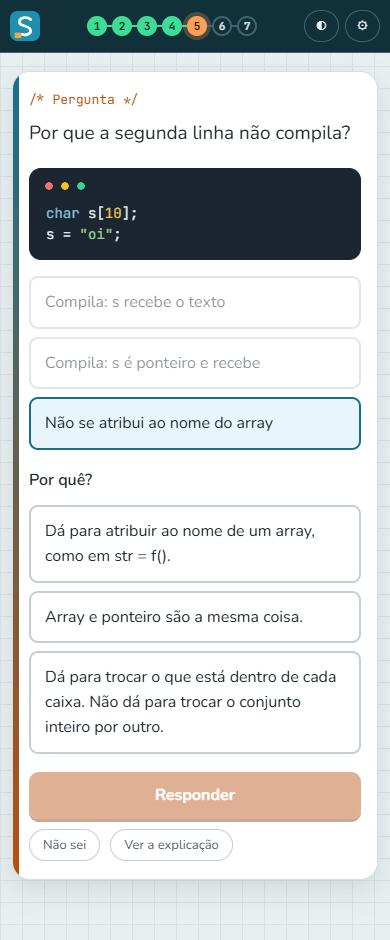
\includegraphics[width=.5\textwidth,height=.55\textheight,keepaspectratio]{fig-3-1-pergunta.jpg}
\fonte{Captura de tela do Structura, elaborada pelo autor.}
\end{figure}

A pergunta de abertura de cada premissa é, de preferência, uma questão com código de nível intermediário: a que pede que a pessoa aplique a ideia num trecho de programa. Questões que usam construções que nenhum tópico ensinou até ali (laço, \texttt{struct}, variável global, entre outras) ficam fora da trilha, para não cobrar o que não foi ensinado; nos 13 tópicos, todas as premissas abrem com uma questão de código.

Do cruzamento dos três sinais saem quatro caminhos (Quadro~\ref{qua:3-2}).

\begin{quadro}[htbp]
\caption{A classificação e o caminho de cada caso}\label{qua:3-2}
\footnotesize
\begin{tabularx}{\textwidth}{|X|X|>{\centering\arraybackslash}p{1.9cm}|}
\hline
\textbf{O que a pessoa fez} & \textbf{Situação} & \textbf{Caminho} \\ \hline
resposta certa, razão certa, ``tenho certeza'' & sabe & firme \\ \hline
certa sem certeza, certa pela razão errada, ou errada pela razão certa & acerto sem firmeza & reforço \\ \hline
``Não sei'', ou errada com ``chutei'' & não sabe & lacuna \\ \hline
errada, pela razão de uma concepção errônea, com alguma certeza & acha que sabe & crença \\ \hline
\end{tabularx}
\fonte{Elaborado pelo autor.}
\end{quadro}

A certeza declarada, aqui, não mede o estado mental da pessoa: ela escolhe o percurso. Quem erra dizendo ``chutei'' sabe que não sabe, e recebe ensino; quem erra com convicção, pela razão de uma concepção mapeada, recebe a demonstração que confronta aquela concepção. A escala tem três pontos porque precisa caber num toque dentro do ritmo da atividade, e o ponto do meio (``acho que sei'') puxa sempre para o lado conservador: não confirma um acerto, e não deixa de tratar uma crença.

\section{A trilha: o percurso de um tópico}

Uma sessão percorre um tópico, premissa por premissa, na ordem do grafo:

\begin{center}\small\ttfamily
entrada~$\rightarrow$~premissa~1~$\rightarrow$~premissa~2~$\rightarrow$~…~$\rightarrow$~reconferência~$\rightarrow$~fechamento
\end{center}

Cada premissa recebe no máximo um trabalho (o da lacuna ou o da crença), o que garante um teto para a duração da sessão. Os quatro caminhos funcionam assim:

\begin{itemize}
\item \textbf{Firme.} Um retorno curto, que diz por que a resposta está certa (cada uma das 79 perguntas de abertura tem essa explicação escrita, para que o acerto também ensine) e, no ritmo ``completo'', uma segunda pergunta de outra natureza: depois de marcar, a pessoa escreve: é o passo de produzir mais alto da escada da premissa (3.4). Acertou, a premissa fecha como ``já sabia''. No ritmo ``rápido'', a resposta firme fecha sozinha.
\item \textbf{Reforço.} Uma pergunta a mais, em outro formato. Certa e pela razão certa, a premissa fecha como ``firmou''; senão, segue o trabalho que a nova resposta pedir.
\item \textbf{Lacuna.} A pessoa sobe a escada da premissa: os passos guiados e um passo de prática, com retorno imediato a cada um. O passo errado mostra a correção, com a resposta certa, e a subida segue: ninguém fica preso num passo. Um dos passos guiados de cada escada tem, entre as alternativas, a concepção errônea da premissa dita com todas as letras, e pede a certeza (Figura~\ref{fig:3-2}): escolhida com convicção, ela abre a demonstração na hora, porque é o mesmo episódio da pergunta de abertura. A premissa fecha como ``aprendeu agora'' quando a pessoa acerta a pergunta seguinte; se erra, vem a revisão: duas ou três frases com a ideia e um trecho de código, animado pela cena da premissa (3.6).
\item \textbf{Crença.} A tela ``Você disse'' repete a concepção que a pessoa sustentou e pede uma previsão: o que ela espera que o programa faça. A tela seguinte mostra o que a máquina fez (3.5). Depois vem o treino, com os passos de prática da escada; a premissa fecha como ``corrigiu uma ideia'' quando o treino fecha.
\end{itemize}

\begin{figure}[htbp]
\centering
\caption{Um passo guiado da escada, com a concepção errônea entre as alternativas e a certeza (kc\_07 B2, passo 1)}\label{fig:3-2}
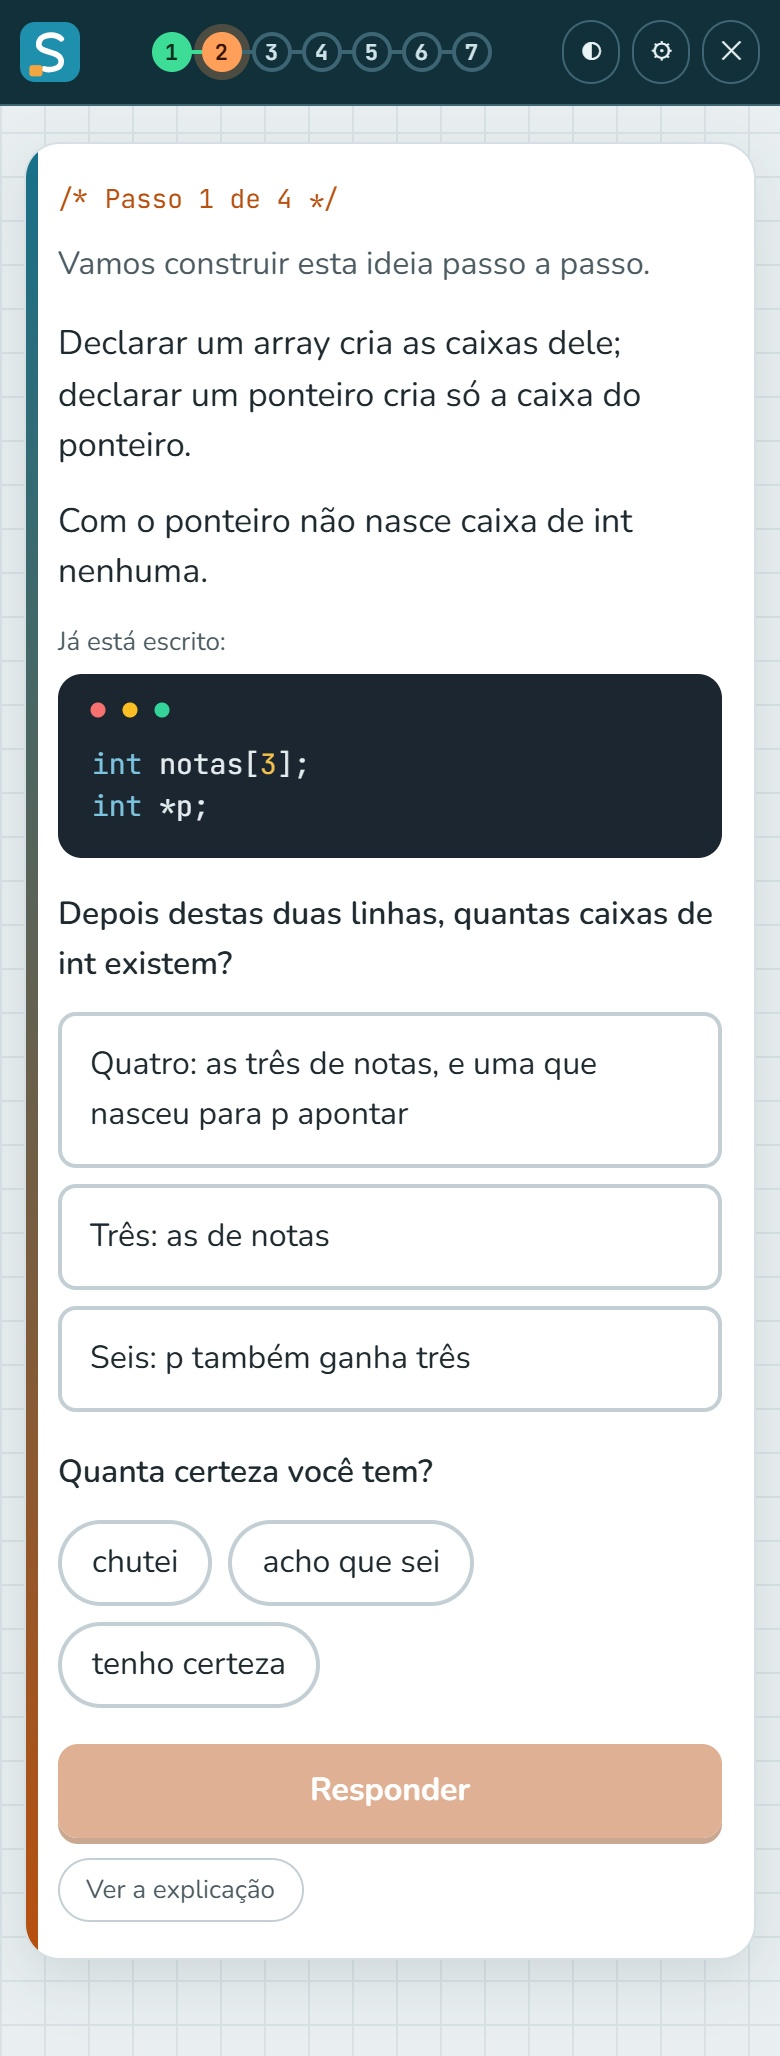
\includegraphics[width=.5\textwidth,height=.55\textheight,keepaspectratio]{fig-3-2-passo.jpg}
\fonte{Captura de tela do Structura, elaborada pelo autor.}
\end{figure}

Depois de todas as premissas, a reconferência faz uma pergunta para cada premissa trabalhada na sessão, ensinada ou corrigida, com outras premissas no meio. É o que separa ``acertou logo depois de ler'' de ``assimilou nesta sessão''. A pergunta é escolhida nesta ordem: o passo em que a pessoa tropeçou, na versão que ela não viu; um passo de produzir ainda não visto; uma questão do banco ainda não usada, que pergunta também a razão; e só então um passo já visto, com outros valores. Quando a razão marcada na reconferência é a concepção que tinha sido corrigida, o fechamento diz que ``a ideia voltou''.

O fechamento (Figura~\ref{fig:3-3}) resume a sessão em quatro blocos (as ideias erradas encontradas e se foram corrigidas; as lacunas, e em que passos; o que já estava firme; e o que ficou em aberto) e, abaixo, mostra a lista de premissas com o resultado de cada uma e o acesso à explicação. O passo em que a pessoa tropeçou aparece pelo nome dele, uma frase curta com a ideia do passo, e não pelo enunciado do exercício.

\begin{figure}[htbp]
\centering
\caption{O fechamento: as ideias erradas encontradas e a situação de cada uma}\label{fig:3-3}
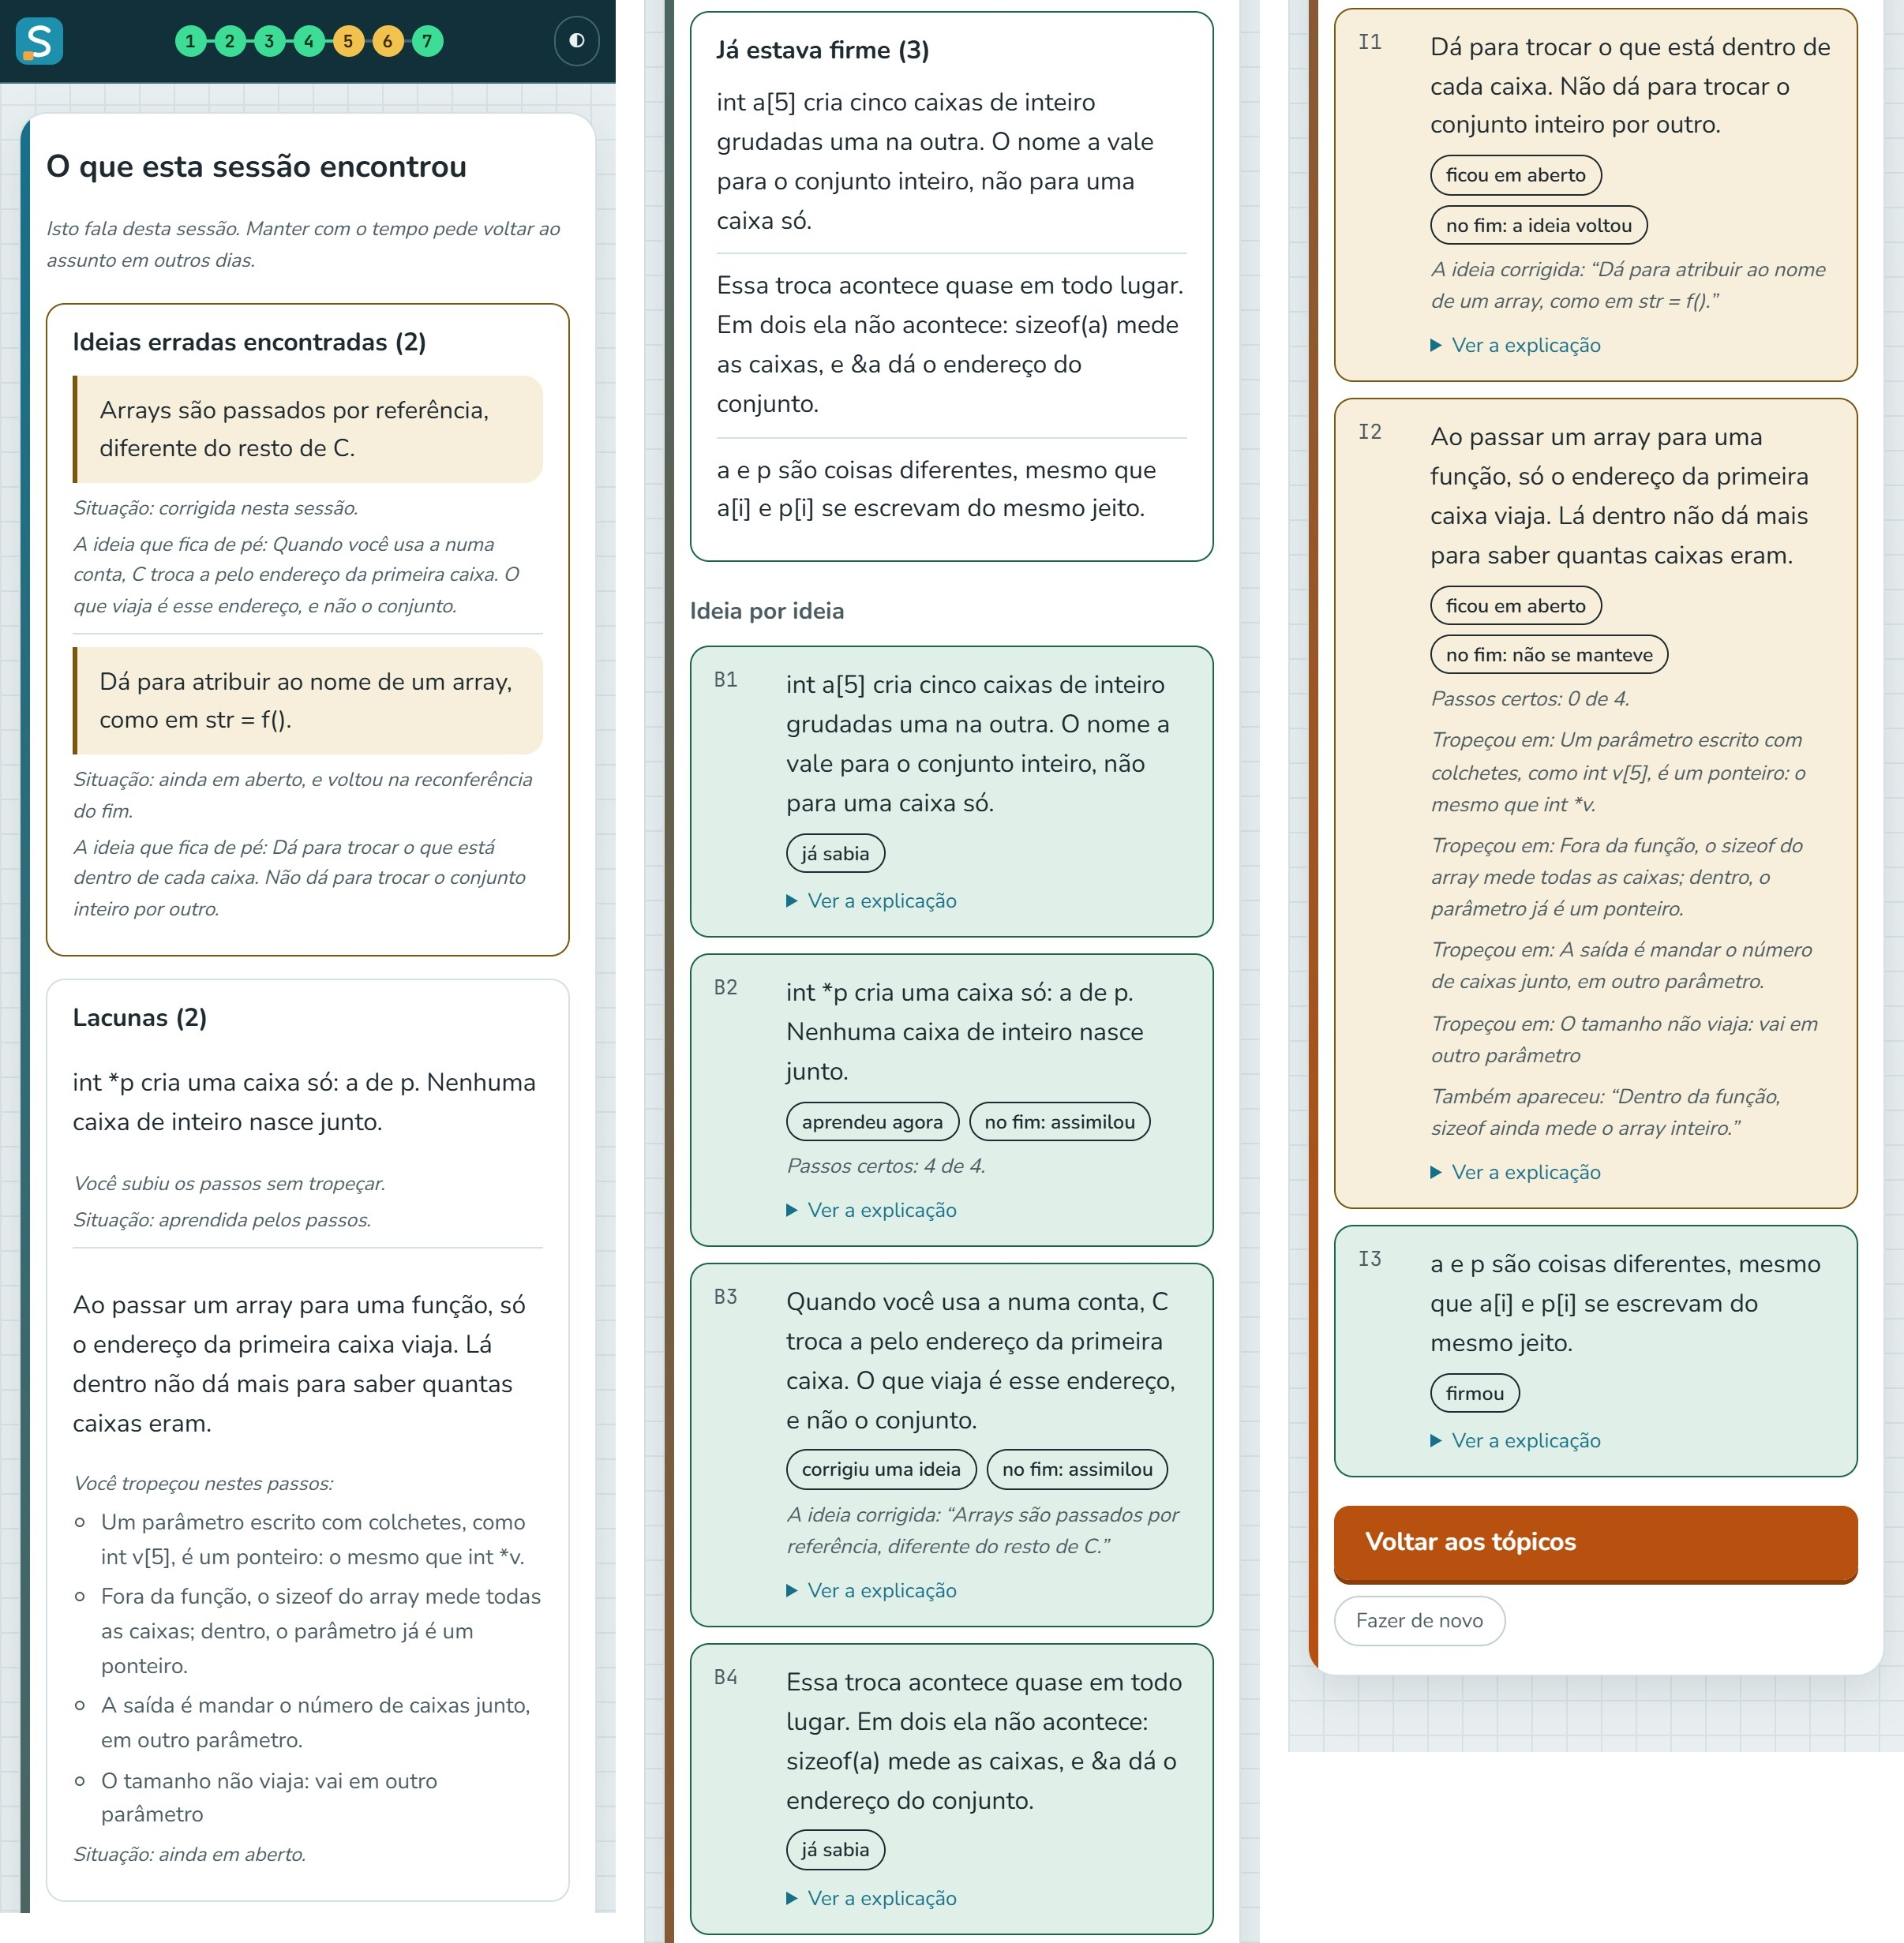
\includegraphics[width=.5\textwidth,height=.55\textheight,keepaspectratio]{fig-3-3-fechamento.jpg}
\fonte{Captura de tela do Structura, elaborada pelo autor.}
\end{figure}

\section{A escada de passos}

Cada premissa tem uma escada: uma sequência ordenada de passos, do mais mecânico até a ideia. Os passos guiados trazem uma ou duas frases curtas e um exercício pequeno; os de prática trazem só o exercício. A mesma escada serve para ensinar (a subida de quem não sabe), para treinar (depois da demonstração) e para reconferir (no fim).

Os exercícios têm cinco formas: tocar a parte de uma linha de código, montar uma linha a partir de peças, escolher entre alternativas, completar a lacuna de uma linha, e digitar a saída de um trecho. Cada passo tem duas versões (a segunda, com outros valores, é a que a reconferência usa), e todo erro previsto tem retorno próprio, que diz o que faltou e mostra o certo. As 79 premissas somam 402 passos (244 guiados e 158 de prática) e 804 versões. As formas se distribuem como no Quadro~\ref{qua:3-3}.

\begin{quadro}[htbp]
\caption{Os passos, por forma}\label{qua:3-3}
\footnotesize
\begin{tabularx}{\textwidth}{|X|l|}
\hline
\textbf{Forma} & \textbf{Passos} \\ \hline
escolher & 190 \\ \hline
digitar & 140 \\ \hline
montar & 37 \\ \hline
completar & 30 \\ \hline
tocar & 5 \\ \hline
\end{tabularx}
\fonte{Elaborado pelo autor.}
\end{quadro}

O texto de cada passo segue uma régua escrita, contra a qual o conteúdo foi revisado: um passo, uma ideia, com no máximo duas frases curtas antes do exercício; só usa o que um passo anterior já ensinou, neste tópico ou num anterior; primeiro o que se faz, depois a ideia; código que um iniciante escreveria; cada passo muda uma coisa só em relação ao anterior; e a analogia, quando há, vem depois do passo, nunca no lugar dele. Cada tópico trabalha as mesmas duas ou três variáveis do começo ao fim (no kc\_10, por exemplo, \texttt{idade} guarda um número, \texttt{p} o endereço de \texttt{idade} e \texttt{pp} o endereço de \texttt{p}), de modo que a declaração cresce e o cenário não muda.

\section{A demonstração com previsão}

Para cada concepção errônea de cada tópico há uma demonstração: um programa curto, de no máximo nove linhas, escrito com os nomes do cenário do tópico, e uma pergunta de previsão com duas alternativas: a que a máquina confirma e a que a concepção errônea espera (Figuras~\ref{fig:3-4}a e~\ref{fig:3-4}b). A pessoa prevê; depois vê o que aconteceu, e uma frase diz o que aquilo mostra e qual premissa fica de pé. As 61 concepções do catálogo dão 80 demonstrações porque 14 delas aparecem em mais de um tópico (a de que o ponteiro é o próprio dado, por exemplo, em quatro), e cada tópico tem a sua, com o cenário dele.

\begin{figure}[htbp]
\centering
\caption{(a) ``Você disse'': a concepção da pessoa e a previsão pedida; (b) ``A máquina respondeu'': o que o compilador disse, a previsão, e a ideia que fica de pé}\label{fig:3-4}
\begin{minipage}[t]{.48\textwidth}\centering
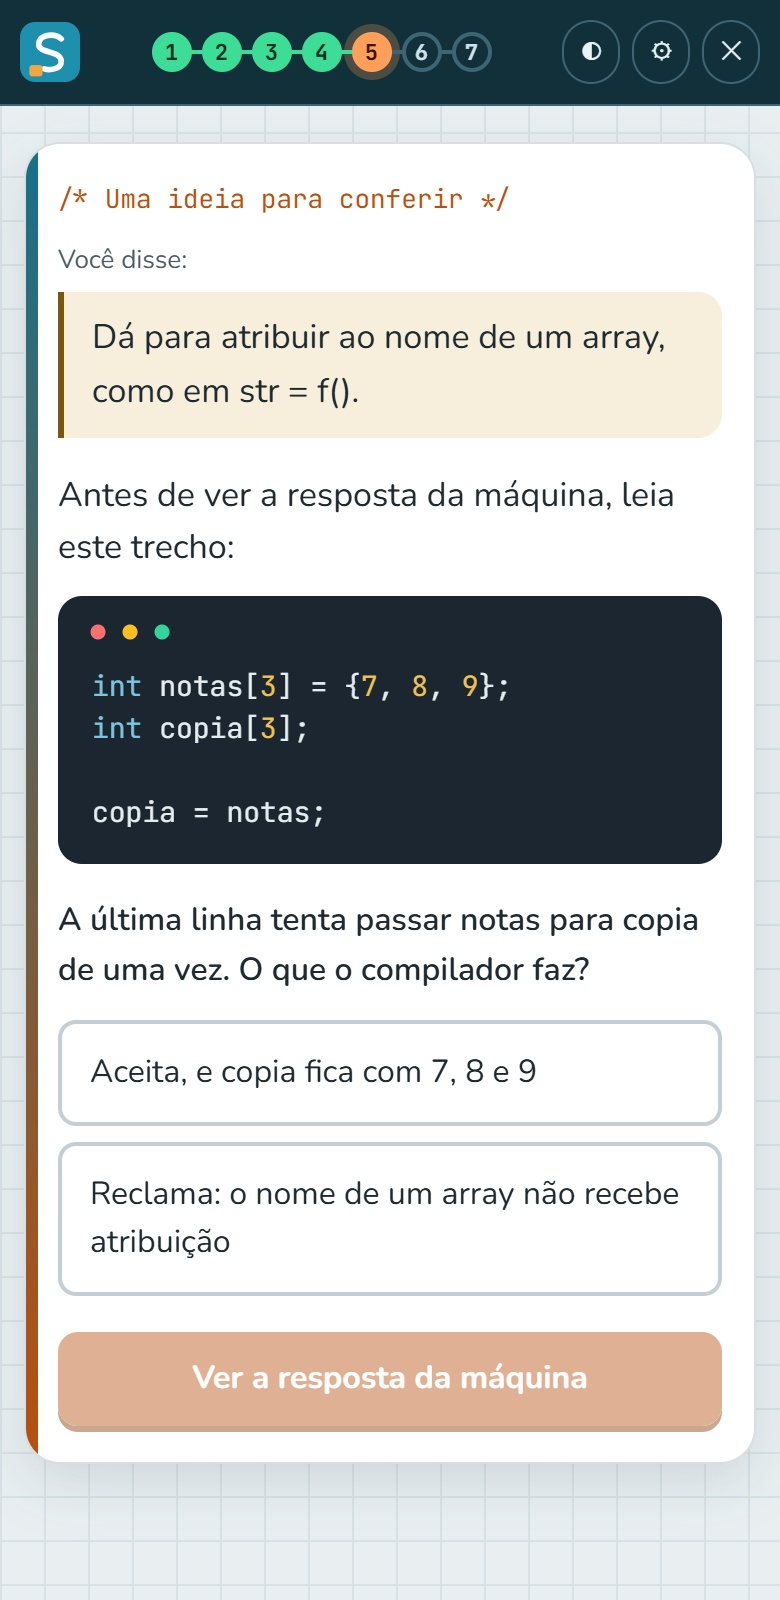
\includegraphics[width=\textwidth,height=.5\textheight,keepaspectratio]{fig-3-4a-voce-disse.jpg}\\[2pt]
(a)
\end{minipage}\hfill
\begin{minipage}[t]{.48\textwidth}\centering
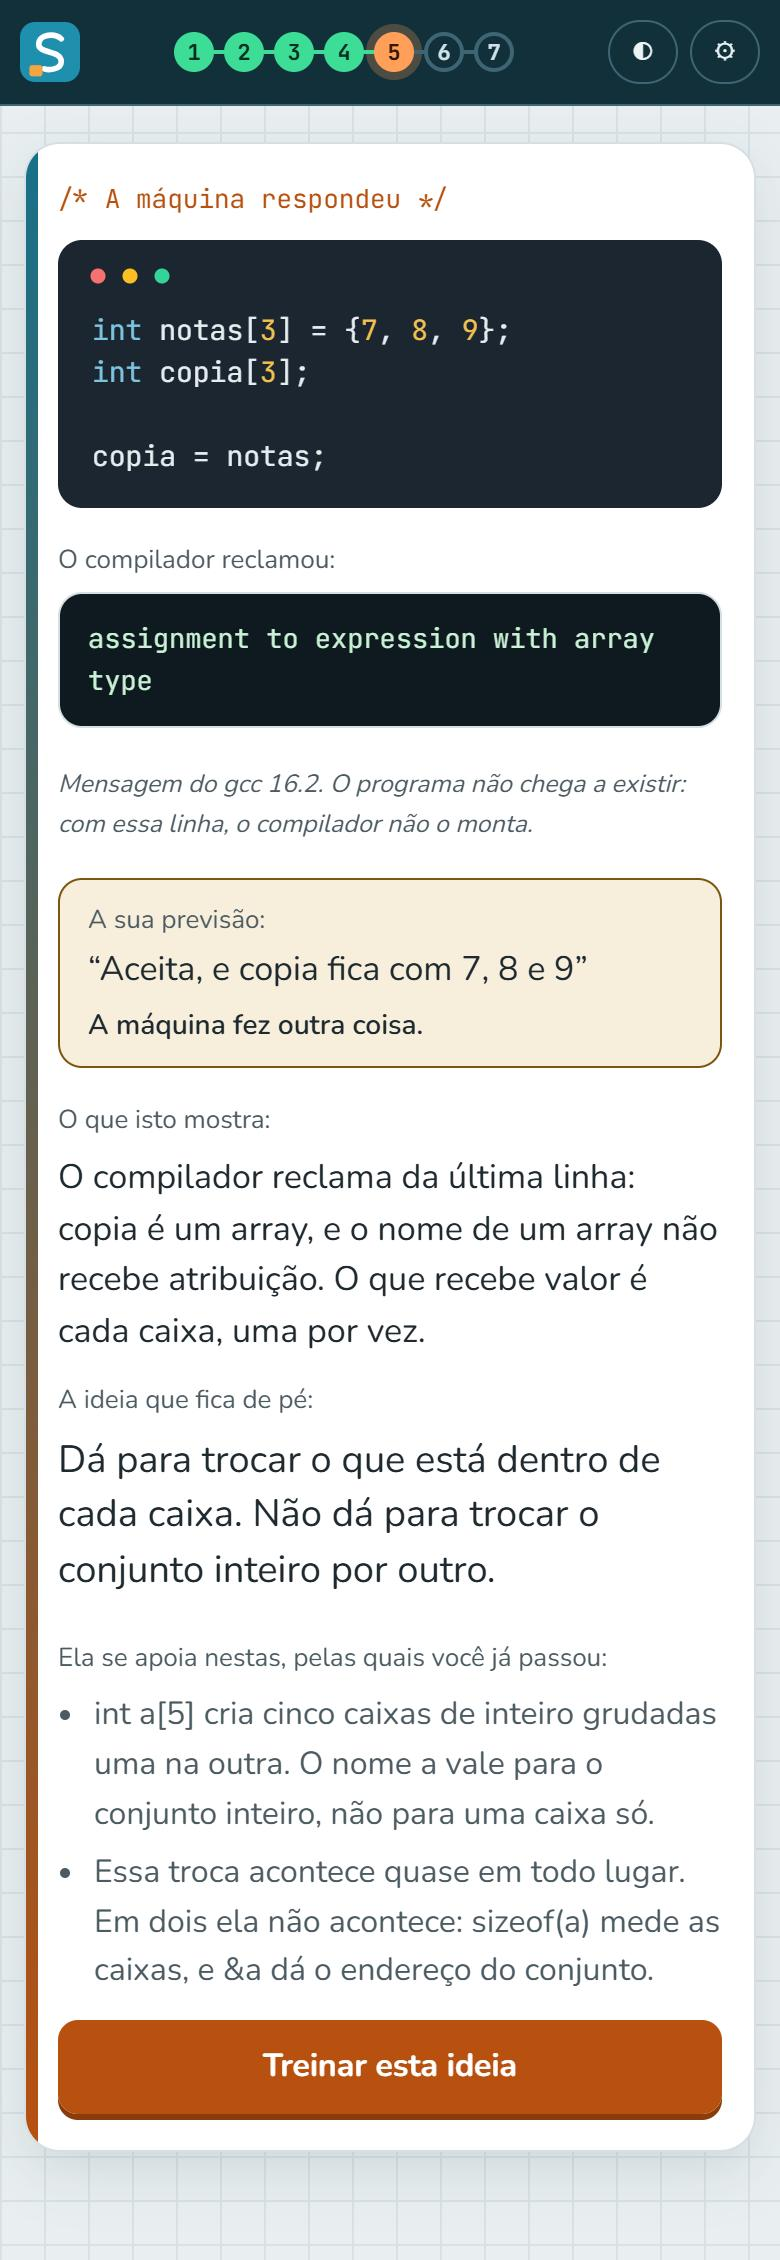
\includegraphics[width=\textwidth,height=.5\textheight,keepaspectratio]{fig-3-4b-maquina.jpg}\\[2pt]
(b)
\end{minipage}
\fonte{Captura de tela do Structura, elaborada pelo autor.}
\end{figure}

O que a máquina ``respondeu'' é de dois tipos. Em 41 das 80 demonstrações é a saída do programa: no kc\_11, por exemplo, quem acredita que a aritmética de ponteiros conta bytes prevê lixo para \texttt{*(p + 3)} sem \texttt{sizeof}, e vê sair o valor de \texttt{notas[3]}. Nas outras 39 é o que o compilador diz do programa: no kc\_12, quem acredita que \texttt{static} muda o escopo de uma variável prevê que o nome \texttt{n} passe a valer fora da função, e vê o compilador reclamar que \texttt{n} não foi declarado ali. Algumas dessas mensagens só aparecem com uma opção a mais do compilador (o analisador de fluxo, \texttt{-{}fanalyzer}, por exemplo, que aponta o bloco de memória pedido e nunca devolvido), e as opções permitidas formam uma lista fechada.

Quando o resultado depende do ambiente (o número de um endereço de memória, o tamanho de um tipo, o comportamento particular de um compilador), a demonstração traz uma nota de ambiente que diz isso com todas as letras. No kc\_12, o gcc 16.2 devolve \texttt{NULL} no lugar do endereço de uma variável local que deixou de existir; a demonstração que usa esse fato diz que é uma escolha do gcc, e que o padrão da linguagem não define aquele valor.

Toda demonstração foi conferida por compilador antes de entrar no sistema: a saída tem de ser a que o texto afirma, e a mensagem tem de sair de uma linha só, porque a tela diz ``o compilador reclamou desta linha'', e a mesma mensagem saindo de duas seria a demonstração dizer menos do que aconteceu. O Capítulo 5 descreve essa conferência.

\section{A cena}

A revisão de cada premissa tem uma cena: o trecho de código dela animado linha a linha (Figura~\ref{fig:3-5}). A linha que roda fica marcada no código, e um palco ao lado mostra o que ela fez: a caixa que nasce, o valor que entra e o que sai, o ponteiro com o seu bilhete, o que vai para a tela. São 79 cenas, uma por premissa.

\begin{figure}[htbp]
\centering
\caption{A cena da revisão do kc\_06 B1, dentro da bancada de \texttt{zera}: a cópia \texttt{n} vira 0, e \texttt{idade} continua 15}\label{fig:3-5}
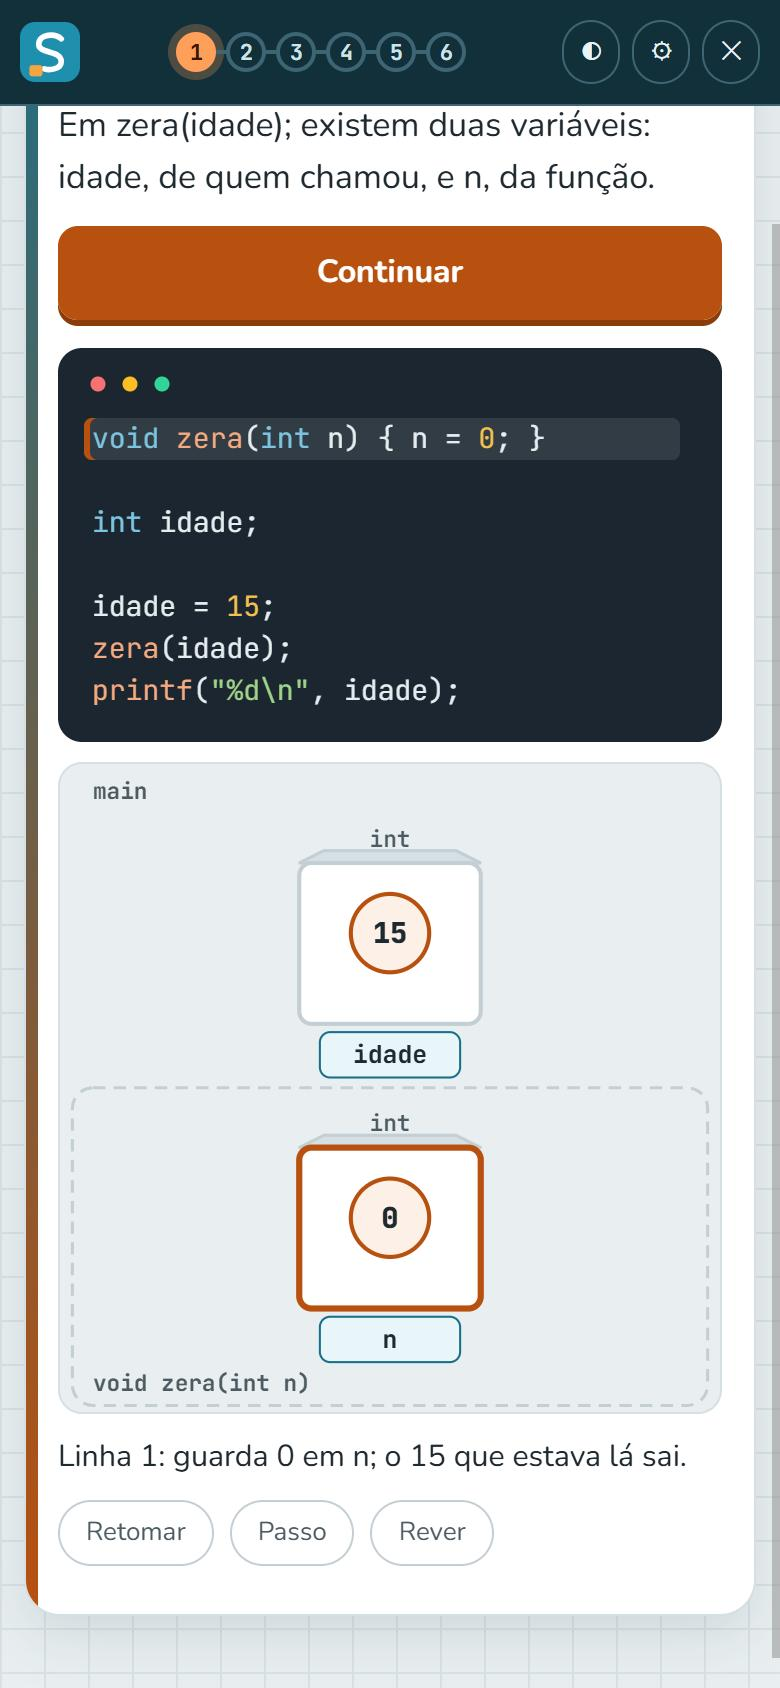
\includegraphics[width=.5\textwidth,height=.55\textheight,keepaspectratio]{fig-3-5-cena.jpg}
\fonte{Captura de tela do Structura, elaborada pelo autor.}
\end{figure}

Os personagens são poucos e vêm da mesma analogia em todos os tópicos. A caixa é a variável: uma etiqueta com o nome, o tipo escrito em cima e o valor numa bolinha dentro, com um ``?'' enquanto não há valor. O ponteiro é uma caixa que guarda um bilhete, ``→ idade'', com uma seta até a caixa apontada; o \texttt{NULL} é o bilhete que diz \texttt{NULL}, sem seta. A fileira é o array: as caixinhas lado a lado, com o índice embaixo, ou em linhas e colunas na matriz, e a caixinha que a linha lê ou escreve fica marcada; o texto entra como uma fileira de \texttt{char} com o \texttt{\textquotesingle{}\textbackslash{}0\textquotesingle{}} no fim. A bancada é a função enquanto roda: um andar próprio, com a primeira linha da função por título, onde nascem as caixas dela, que somem quando ela termina, menos a marcada \texttt{static}, que fica. E o bloco alugado é o que o \texttt{malloc} pede: ele mora num andar à parte, o monte, com a placa ``alugado'', e depois do \texttt{free} fica apagado, com a placa ``devolvido''.

A cena anda sozinha, um passo por segundo e pouco, com os botões Pausar, Passo e Rever. Quem pediu ao sistema operacional menos movimento vê a cena já no estado final, com o passo a passo nos botões. Cada passo tem uma frase, escrita embaixo do palco e lida pelos leitores de tela; por exemplo: ``Linha 3: guarda 21 em idade; o 20 que estava lá sai.'' Em tela de computador, a cena fica ao lado do texto da revisão; no celular, embaixo.

A cena é dado, e não desenho: cada uma é uma lista de passos, um por linha executada, com as ações daquela linha (criar uma caixa, guardar um valor, apontar, chamar e voltar de uma função, alugar e devolver um bloco). Por ser dado, ela é conferida contra o compilador como o resto do conteúdo (Capítulo 5): o palco nunca mostra um valor que o programa não tem.

\section{O registro e a retomada}

Tudo o que a pessoa faz é gravado num registro só de acréscimo, um evento por linha: a resposta, a razão, a certeza, o tempo, a previsão e se ela coincidiu com a concepção errônea, os passos errados, a reconferência. Nada é apagado ou reescrito. A sessão inteira pode ser reconstruída reexecutando as entradas gravadas: é assim que o sistema retoma uma sessão depois de o servidor reiniciar, e é por isso que tudo o que muda o caminho da sessão é entrada registrada. Como uma mudança nas regras faria as mesmas respostas caírem em telas diferentes, a primeira linha de cada sessão diz a versão das regras com que ela começou, e uma sessão de outra versão não é refeita: a pessoa vê uma mensagem, e não uma tela errada.

A identificação é por um código de participante, opcional e sem nenhum dado pessoal; o mesmo código retoma a sessão no mesmo tópico. Sem código, é o navegador que guarda o número da sessão: quem fecha a página e reabre o tópico volta à tela em que estava.

No meio da sessão, o botão Sair do topo oferece duas saídas. ``Guardar e sair'' volta à página dos tópicos, e a sessão continua de onde parou quando o tópico é reaberto. Não há o que gravar a mais, porque cada resposta já está no registro. ``Cancelar a sessão'', depois de uma confirmação, faz o tópico recomeçar do zero. Também o cancelamento não apaga nada: o registro ganha uma linha dizendo que a sessão foi cancelada, e daí em diante ela não é mais retomada: nem pelo número, nem pelo código, nem refeita depois de um reinício do servidor.

\section{A interface}

A interface foi desenhada para parecer um ambiente de programação, em dois temas: o escuro, inspirado num editor de código à noite (Figura~\ref{fig:3-6}), e o claro, com o topo escuro como a barra de um terminal (Figuras~\ref{fig:3-1} a~\ref{fig:3-4}). O tema é escolhido antes de a página ser desenhada (o do sistema operacional, ou o que a pessoa escolheu da última vez), e pode ser trocado por um botão no topo. Todos os pares de texto sobre fundo passam na razão de contraste de 4,5:1 que o critério 1.4.3 da WCAG 2.1, no nível AA, exige para texto comum \cite{w3c2025}, nos dois temas; quem pediu ao sistema operacional menos movimento não vê animação.

O código aparece numa moldura de editor, com cores por categoria (palavras-chave, números, textos, comentários, nomes de função); a saída do programa e a mensagem do compilador aparecem numa moldura de terminal, sem cores de código. O topo da trilha mostra o tópico e uma parada por premissa, numerada, com o estado de cada uma (feita, em aberto, agora ou ainda não), também dito em texto para leitores de tela, além dos botões de tema, de ajustes (o ritmo) e de sair. Em tela de celular os botões ficam só com o desenho, para que as oito paradas do kc\_09 caibam em 360 px de largura.

A página inicial desenha o caminho dos 13 tópicos como a trilha de um jogo (Figura~\ref{fig:3-6}): dez tópicos em fila, do kc\_00 ao kc\_09 (com o kc\_01, modelo de memória, depois do kc\_06 e do kc\_07), abrindo-se em três no fim (kc\_10, kc\_11 e kc\_12, que não dependem um do outro). A ordem é sugerida, e não imposta: todos os tópicos ficam abertos, e um teste confere que cada tópico vem depois dos seus pré-requisitos. Cada parada mostra o seu estado (já feito, próximo, em andamento ou aberto) e o andamento do tópico (``3 de 6''), e o próximo sugerido aparece num cartão acima do caminho.

\begin{figure}[htbp]
\centering
\caption{A página inicial no tema escuro: o próximo sugerido e o caminho dos 13 tópicos, com um tópico feito e um em andamento}\label{fig:3-6}
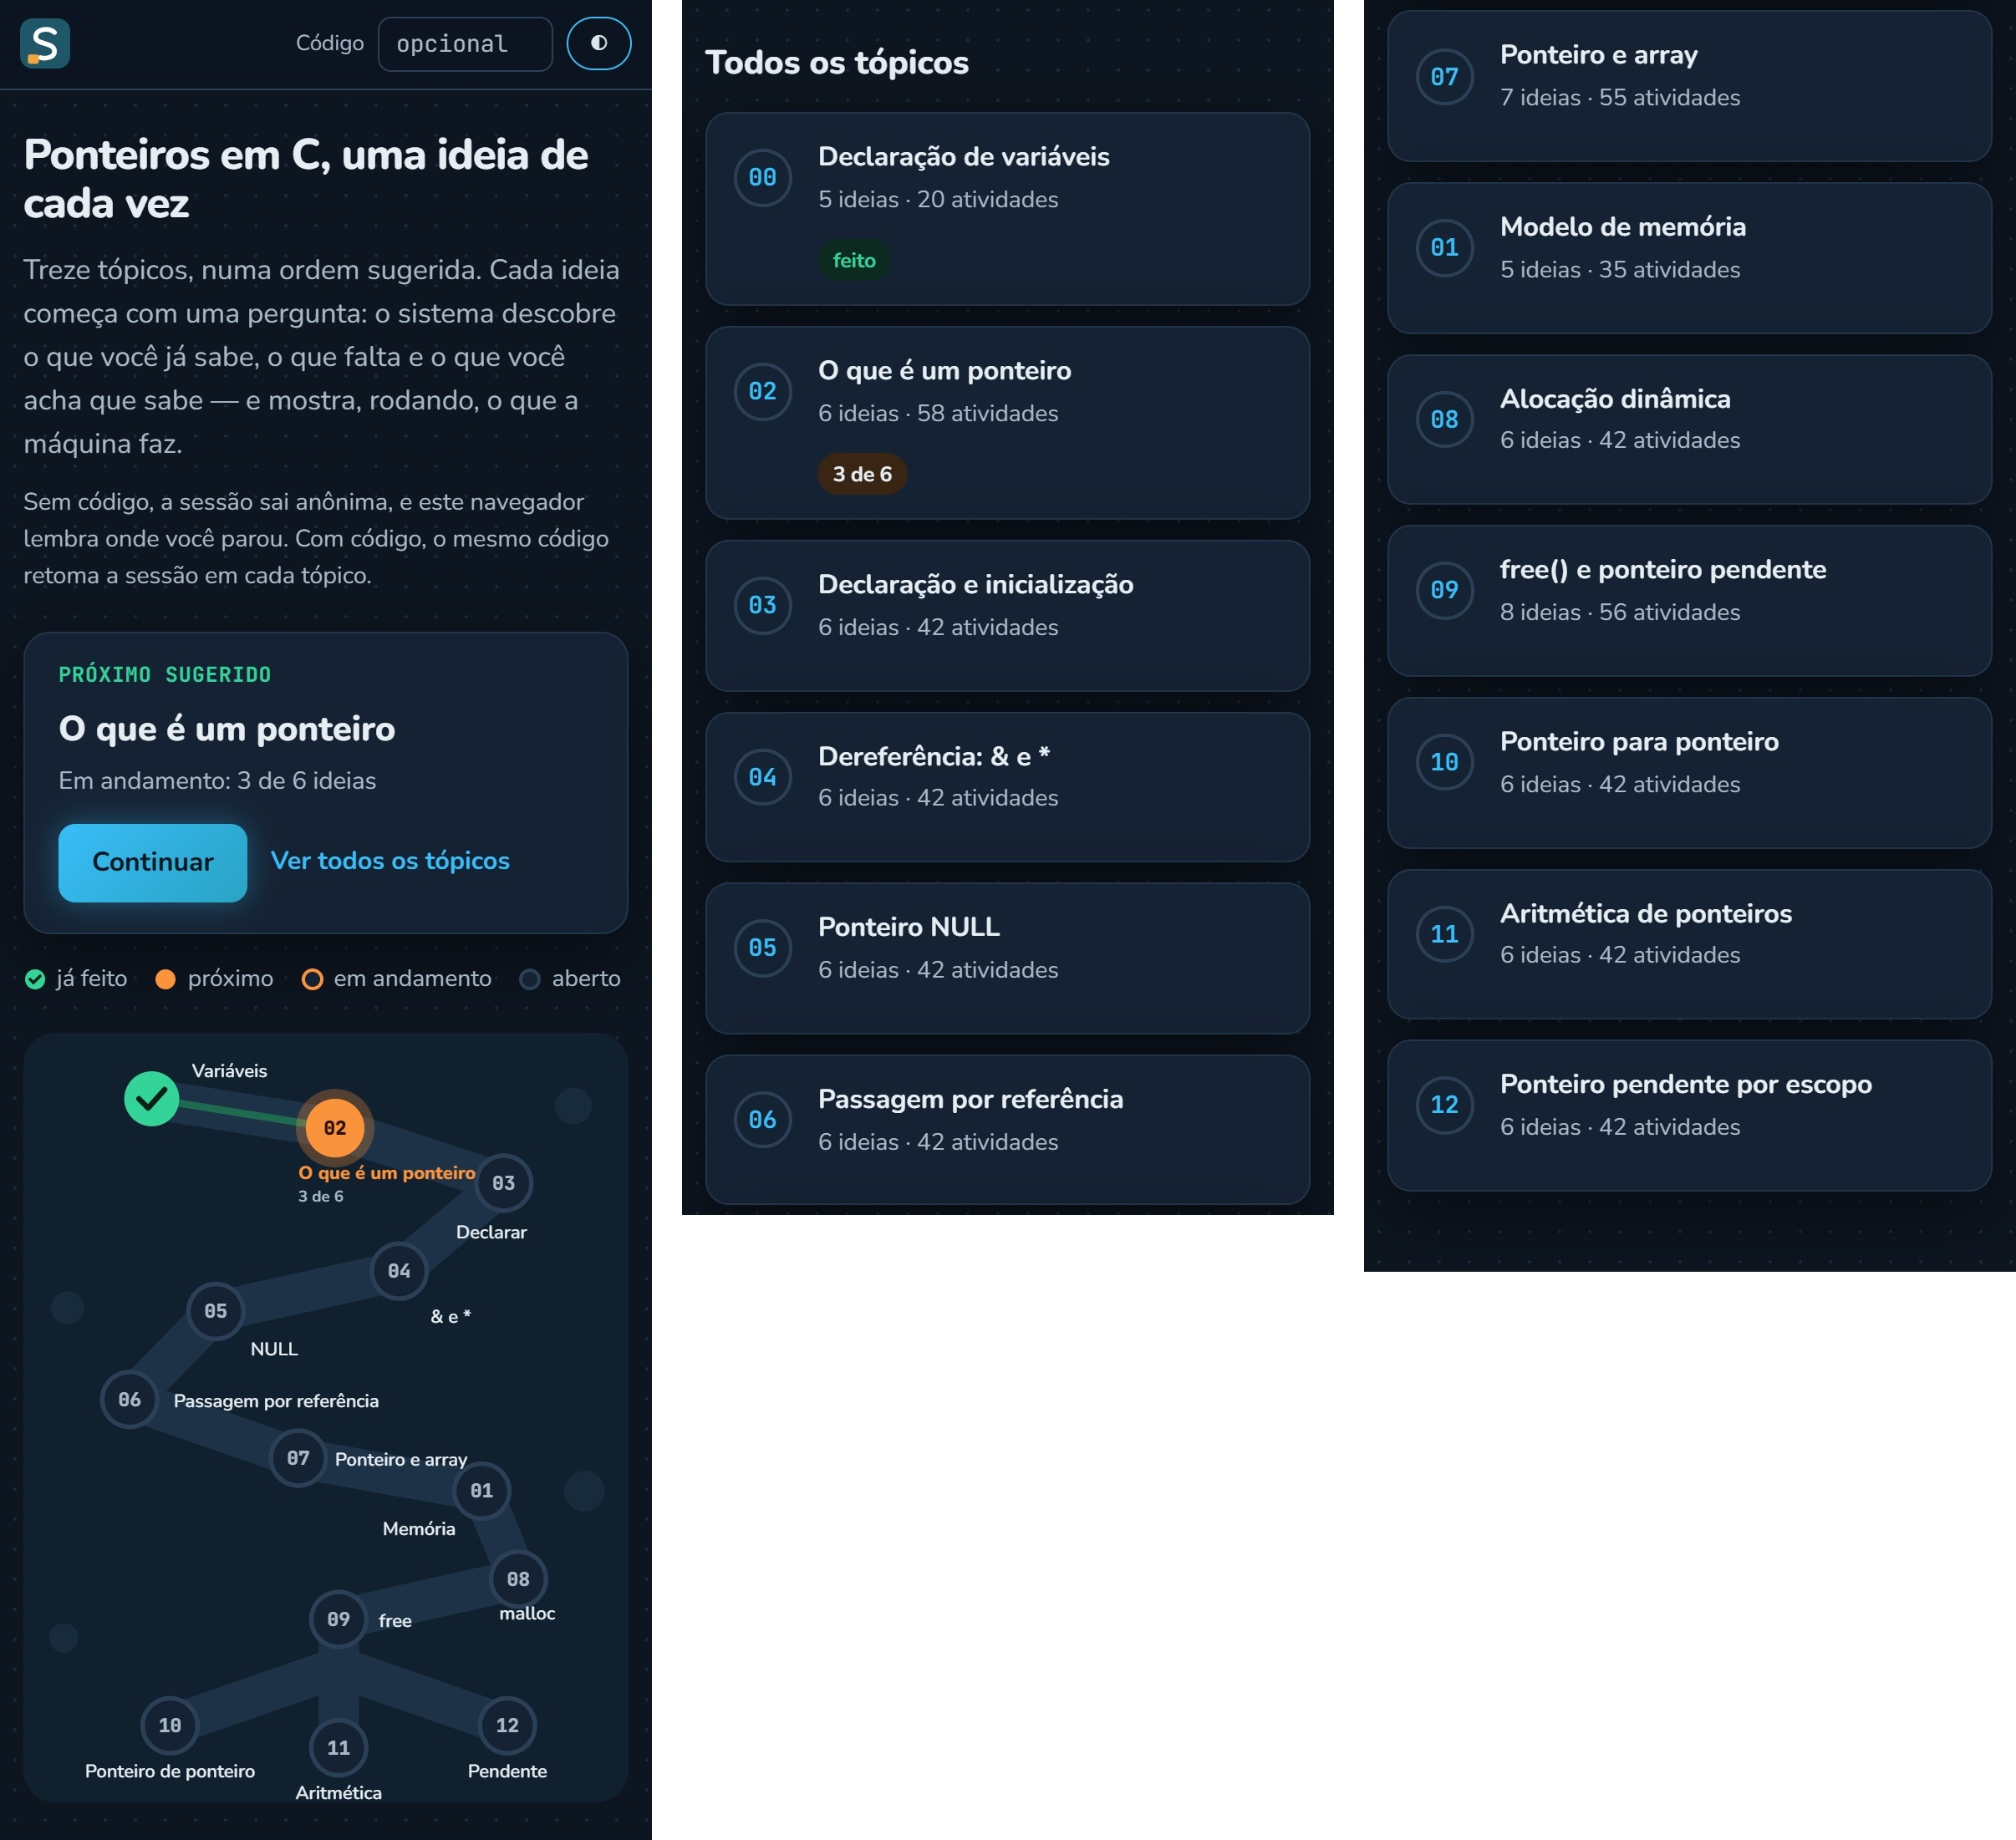
\includegraphics[width=.5\textwidth,height=.55\textheight,keepaspectratio]{fig-3-6-inicio-escuro.jpg}
\fonte{Captura de tela do Structura, elaborada pelo autor.}
\end{figure}

As fontes são livres (licença OFL) e estão guardadas no próprio projeto: nenhuma página carrega nada de outro endereço.

\section{Arquitetura}

O sistema é escrito em Python, com um servidor HTTP (FastAPI) e páginas em HTML, CSS e JavaScript sem dependências externas. O conteúdo (premissas, concepções errôneas, questões e escadas) fica em arquivos YAML, separados do código: acrescentar ou corrigir conteúdo não exige mexer no motor. O motor da trilha é uma função pura do estado da sessão e da entrada da pessoa, que devolve a próxima tela; é isso que torna a sessão reexecutável a partir do registro. Um portal monta os 13 tópicos num só servidor, que roda num contêiner Docker na própria máquina do laboratório, sem depender de serviço externo.

	% Gerado de docs/monografia/curadoria.md por scripts/monografia_latex.py.
% Não edite aqui: edite o .md e gere de novo.

\chapter{\texorpdfstring{\mbox{CURADORIA} \mbox{DO} \mbox{CATÁLOGO} \mbox{DE} \mbox{CONCEPÇÕES} \mbox{ERRÔNEAS}}{CURADORIA DO CATÁLOGO DE CONCEPÇÕES ERRÔNEAS}}\label{cap:4}

\section{Problema da procedência}

O sistema descrito nos capítulos anteriores formula, a cada atividade respondida, uma hipótese com consequência imediata: a de que a pessoa provavelmente sustenta determinada concepção errônea. É essa hipótese que seleciona o percurso de refutação a ser apresentado.

A validade da hipótese depende de uma questão anterior, que o software não responde: a origem de cada concepção do catálogo. Se uma concepção tiver sido incluída apenas por parecer plausível ao autor, o sistema não estará diagnosticando uma concepção errônea documentada, e sim produzindo dados sobre uma suposição, com a mesma aparência de rigor do restante. Por essa razão, o projeto adota a seguinte regra: uma concepção sem procedência é tratada como hipótese do autor e não é incluída no catálogo como achado.

Este capítulo trata dessa questão, que pode ser verificada sem a participação de estudantes. O instrumento não foi avaliado com estudantes, limitação declarada no Capítulo 7. O que se sustenta aqui é mais restrito e inteiramente verificável: o sistema afirma sobre concepções errôneas apenas o que a literatura registra e identifica explicitamente os casos em que não há registro.

\section{Graus de procedência}

Cada concepção do catálogo possui um campo de procedência (\texttt{provenance}), que assume um de cinco valores. O grau não descreve a importância da concepção nem a confiança do autor nela: descreve o tipo de obra que a sustenta (Quadro~\ref{qua:4-1}).

\begin{quadro}[htbp]
\caption{Graus de procedência}\label{qua:4-1}
\footnotesize
\begin{tabularx}{\textwidth}{|l|X|}
\hline
\textbf{grau} & \textbf{significado} \\ \hline
\texttt{D} & documentada: achado empírico, com fonte e posição localizável \\ \hline
\texttt{L} & registrada como erro comum em obra técnica \\ \hline
\texttt{T} & transposta de outra linguagem, com a analogia declarada \\ \hline
\texttt{N} & o erro consta de norma, como o padrão de codificação CERT C \cite{sei2025} e a CWE, \textit{Common Weakness Enumeration} \cite{mitre2026}, mas a concepção não \\ \hline
\texttt{E} & elaborada a partir do modelo de máquina: hipótese a testar \\ \hline
\end{tabularx}
\fonte{Elaborado pelo autor.}
\end{quadro}

Duas propriedades desse campo são relevantes para o método.

A primeira é que o grau constitui uma afirmação sobre a literatura, e não sobre o uso da concepção no sistema. Uma mesma concepção pode aparecer em mais de um tópico do domínio (o que ocorre com quatorze delas), e o texto que a contextualiza varia de um tópico para outro; o grau, porém, deve ser o mesmo. Se uma concepção tem grau \texttt{D} em um tópico e \texttt{L} em outro, uma das duas afirmações é falsa, e essa diferença corresponde, em um trabalho acadêmico, à diferença entre citar e alegar. A auditoria encontrou três casos desse tipo (Seção 4.6.5), e um teste automatizado impede a divergência (Quadro~\ref{qua:4-7}).

A segunda é que o grau \texttt{E} é legítimo, desde que declarado. Uma hipótese do autor pode integrar o catálogo, mas não pode ser apresentada como achado. As três hipóteses do catálogo são identificadas como tais no próprio campo de fonte, e dois testes independentes asseguram que nenhuma delas apareça nos tópicos selecionados para a coleta de dados.

\section{Classes de fonte}

O catálogo apoia-se em dois tipos de obra. A diferença entre eles não é de qualidade, mas do tipo de afirmação que cada um sustenta. Tratá-los como equivalentes constituiria um defeito metodológico; a declaração da classe, concepção por concepção, é o que torna o catálogo auditável.

\subsection{Classe 1: literatura de concepções errôneas (23 concepções)}

A primeira classe compreende estudos empíricos com estudantes e revisões que os agregam. A obra principal é o Apêndice A de \citeonline{sorva2012}, cuja Tabela A.1 relaciona 162 concepções errôneas levantadas na literatura de ensino de programação introdutória, cada uma com tópico, descrição e fonte. A ela se somam os estudos que a própria tabela atribui: du Boulay (\citeyear{duboulay1986}), \citeonline{soloway1982}, \citeonline{putnam1986}, \citeonline{sleeman1986}, \citeonline{samurcay1989}, \citeonline{holland1997}, \citeonline{ma2007}, \citeonline{doukakis2007} e \citeonline{kaczmarczyk2010}. Uma obra externa à Tabela A.1 também sustenta uma das concepções: \citeonline{hermans2018} registram a ideia de que a variável armazena vários valores ou ``lembra'' os anteriores e a investigam em um experimento com 496 iniciantes.

Essa classe sustenta que a concepção foi observada em estudantes por pesquisadores que a investigaram.

\subsection{Classe 2: corpus de praticante (34 concepções)}

A segunda classe é constituída pelo FAQ (\textit{Frequently Asked Questions}, perguntas frequentes) do grupo comp.lang.c, compilado em 1990 a partir do grupo de Usenet de mesmo nome, aprimorado de forma episódica desde então e publicado em livro por \citeonline{summit1996}.

A inclusão dessa classe requer justificar por que um FAQ de linguagem constitui evidência sobre concepções errôneas, e não apenas sobre a linguagem C. A justificativa está no critério de inclusão adotado, que pode ser conferido por qualquer leitor: é incluída somente a pergunta cujo título enuncia a concepção na voz de quem a sustenta, em primeira pessoa (Quadro~\ref{qua:4-2}).

\begin{quadro}[htbp]
\caption{Exemplos de perguntas do FAQ cujo título enuncia a concepção na voz de quem a sustenta}\label{qua:4-2}
\footnotesize
\begin{tabularx}{\textwidth}{|l|X|}
\hline
\textbf{pergunta} & \textbf{título} \\ \hline
6.2 & ``But I heard that \texttt{char a[]} was identical to \texttt{char *a}.'' \\ \hline
6.9 & ``Someone explained to me that arrays were really just constant pointers.'' \\ \hline
6.4b & ``So arrays are passed by reference, even though the rest of C uses pass by value?'' \\ \hline
4.11 & ``Does C even have ``pass by reference''?'' \\ \hline
\end{tabularx}
\fonte{Elaborado pelo autor, com títulos de perguntas de \citeonline{summit1996}.}
\end{quadro}

O catálogo, portanto, não infere a concepção a partir de uma explicação técnica: registra a formulação de quem a sustenta. Para conferir a inclusão, basta consultar a pergunta e avaliar se o título enuncia a concepção ou apenas o assunto.

Do ponto de vista metodológico, o FAQ é tratado como fonte documental: um corpus de confusões autorrelatadas, de ocorrência natural, selecionadas por recorrência ao longo de mais de três décadas. O tratamento dado a esse corpus é o da análise documental.

Essa classe sustenta que a confusão ocorre e é recorrente entre aprendizes da linguagem C. Não sustenta afirmações de prevalência: a população é autosselecionada (pessoas que escrevem para um grupo de Usenet), e a frequência das perguntas reflete o julgamento do editor, e não uma medição. Por isso, nenhuma afirmação de proporção é extraída dessa fonte.

\subsection{Necessidade da segunda classe}

Seria razoável exigir que todo o catálogo se apoiasse na classe 1, de natureza empírica, e que a classe 2 fosse dispensada. Essa exigência foi testada contra a Tabela A.1 de \citeonline{sorva2012}, item por item, e verificou-se que não pode ser satisfeita.

A Tabela A.1 possui um tópico dedicado a referências (\texttt{Refs}, com 17 dos 162 itens) e itens sobre memória e tempo de vida distribuídos pelos tópicos \texttt{VarAssign}, \texttt{ObjState} e \texttt{Misc}. Faltam-lhe, contudo, os itens relevantes para este trabalho, como mostra a contagem do Quadro~\ref{qua:4-3}, reprodutível por busca de termos no texto da tabela.

\begin{quadro}[htbp]
\caption{Ocorrências de termos relativos à memória na Tabela A.1}\label{qua:4-3}
\footnotesize
\begin{tabularx}{\textwidth}{|X|X|}
\hline
\textbf{termo buscado na Tabela A.1} & \textbf{ocorrências} \\ \hline
\texttt{malloc}, \texttt{free}, \texttt{deallocat}, \texttt{garbage} & 0 \\ \hline
\texttt{heap}, \texttt{stack} & 0 \\ \hline
\texttt{arithmetic}, \texttt{decay}, \texttt{dangling}, \texttt{sizeof} & 0 \\ \hline
\texttt{null} & 1: o item 54, ``Null model of recursion'' \cite[p.~362]{sorva2012}, que não trata de ponteiro nulo \\ \hline
\texttt{lifetime} & 1: o item 5, ``Difficulties understanding the lifetime of values'' \cite[p.~359]{sorva2012} \\ \hline
\texttt{memory} & 7 \\ \hline
\end{tabularx}
\fonte{Elaborado pelo autor, por busca no texto de \citeonline{sorva2012}.}
\end{quadro}

Não há, portanto, nenhum item sobre \texttt{NULL}, sobre \texttt{malloc} e \texttt{free}, sobre aritmética de ponteiros, sobre decaimento de array ou sobre a distinção entre pilha e monte.

Essa ausência não decorre de descuido da obra: o catálogo de \citeonline{sorva2012} refere-se à programação introdutória em Java, Python e BASIC, linguagens em que esses construtos não existem. A literatura de concepções errôneas produzida nessas linguagens não poderia documentar confusões relativas justamente ao que distingue a linguagem C.

Conclui-se, assim, não que as 34 concepções da classe 2 sejam frágeis, mas que um catálogo de concepções errôneas para C requer uma segunda classe de fonte, a qual deve ser declarada como tal, com a indicação do que sustenta e do que não sustenta. Essa declaração é feita, concepção por concepção, na coluna de classe do Apêndice B.

\section{Procedimento de conferência}

O padrão adotado pelo projeto, registrado no cabeçalho do primeiro catálogo de tópico, é o de que as fontes sejam conferidas na obra primária, e não citadas de memória. O resultado da aplicação desse padrão a cada concepção é apresentado no Quadro~\ref{qua:4-4}.

O quadro é exaustivo e mutuamente exclusivo: cada uma das 61 concepções figura em exatamente uma linha, que registra a verificação mais forte obtida para ela. A soma é, por construção, igual a 61. Um quadro que contasse as concepções que citam cada obra teria soma maior, pois uma concepção pode citar mais de uma obra, e não permitiria determinar quantas ficaram sem conferência.

\begin{quadro}[htbp]
\caption{Forma de conferência de cada uma das 61 concepções}\label{qua:4-4}
\footnotesize
\begin{tabularx}{\textwidth}{|X|l|}
\hline
\textbf{forma de conferência} & \textbf{concepções} \\ \hline
conferida no texto integral de \citeonline{sorva2012}, obtido do repositório aberto da Universidade Aalto (handle \texttt{123456789/3534}, bundle TEXT); a frase em inglês citada entre aspas foi localizada no texto da obra & 21 \\ \hline
conferida no índice do FAQ comp.lang.c: as seções 1, 4, 5, 6 e 7 foram consultadas em \texttt{c-{}faq.com}; as perguntas citadas existem, e os títulos coincidem com os citados no catálogo & 32 \\ \hline
citação abreviada no catálogo, com a forma integral localizada na obra & 1 \\ \hline
cita \citeonline{sorva2012} com página e item, mas sem frase entre aspas, o que impede a verificação pelo procedimento automatizado & 1 \\ \hline
conferência parcial: a seção 11 do FAQ não foi incluída na curadoria & 1 \\ \hline
não conferida na curadoria: cita apenas normas (CERT C e CWE), conferidas à parte (Seção 4.7) & 1 \\ \hline
sem item correspondente na literatura, com a busca declarada em campo próprio & 2 \\ \hline
sem fonte, por definição: hipótese declarada como tal & 2 \\ \hline
total & 61 \\ \hline
\end{tabularx}
\fonte{Elaborado pelo autor.}
\end{quadro}

As duas primeiras linhas somam as 53 concepções conferidas na obra primária. As seis últimas correspondem ao que a curadoria não afirma ter conferido, com a respectiva justificativa.

Os estudos agregados pelo Apêndice A de \citeonline{sorva2012}, a saber, du Boulay (\citeyear{duboulay1986}), \citeonline{samurcay1989}, \citeonline{sleeman1986}, \citeonline{soloway1982}, \citeonline{putnam1986}, \citeonline{doukakis2007}, \citeonline{ma2007} e \citeonline{kaczmarczyk2010}, não figuram em linha própria porque não foram consultados diretamente. As cinco concepções que os citam fazem-no \textit{apud} \citeonline{sorva2012}, com página e item, e estão contadas na primeira linha do quadro. A Seção 4.7 detalha esse ponto.

A conferência é automatizada sempre que possível: o programa que gera o Apêndice B extrai a frase entre aspas de cada citação e a procura no texto da obra, de modo que o resultado não depende do que está declarado no campo de fonte. Quando o programa é executado sem o texto da obra, o número de concepções conferidas cai de 53 para 32, e o apêndice passa a indicar, linha por linha, que a conferência não foi realizada.

\section{Resultado da curadoria}

O Quadro~\ref{qua:4-5} sintetiza o resultado da curadoria.

\begin{quadro}[htbp]
\caption{Resultado da curadoria}\label{qua:4-5}
\footnotesize
\begin{tabularx}{\textwidth}{|X|X|}
\hline
\textbf{indicador} & \textbf{valor} \\ \hline
concepções distintas no catálogo & 61 \\ \hline
conferidas na obra primária & 53 \\ \hline
graus & \texttt{D} 6, \texttt{L} 33, \texttt{T} 16, \texttt{N} 3, \texttt{E} 3 \\ \hline
hipóteses \texttt{E} & 3, todas fora dos tópicos selecionados para a coleta \\ \hline
\end{tabularx}
\fonte{Elaborado pelo autor.}
\end{quadro}

\section{Achados da auditoria}

Os achados descritos nesta seção têm interesse que ultrapassa o catálogo, pois dizem respeito ao método de construção de um catálogo a partir da literatura, e não à linguagem C.

\subsection{Buscas realizadas com vocabulário ou item inadequado}

Em três concepções, a busca inicial na obra não localizou o item correspondente, embora ele existisse (Quadro~\ref{qua:4-6}).

\begin{quadro}[htbp]
\caption{Buscas que não localizaram o item e o item existente na obra}\label{qua:4-6}
\footnotesize
\begin{tabularx}{\textwidth}{|X|X|X|}
\hline
\textbf{concepção} & \textbf{registro anterior no catálogo} & \textbf{item existente na obra} \\ \hline
\texttt{pointer\_\allowbreak{}has\_\allowbreak{}no\_\allowbreak{}address} & ``procurei no catálogo do Sorva e não está lá: nenhum dos 162 itens afirma que a referência não ocupa espaço'' & a segunda frase do item 14: ``It is not stored inside the computer'' \cite[p.~360]{sorva2012}. A busca utilizou os termos ``referência'' e ``espaço'', ao passo que o item trata de variável \\ \hline
\texttt{array\_\allowbreak{}confused\_\allowbreak{}with\_\allowbreak{}cell} & ``não tem fonte empírica, entra como hipótese'' & o item 151, ``Confusion between an array and its cell'' \cite[p.~367]{sorva2012}, e o item 9, ``A variable can hold multiple values at a time'' \cite[p.~359]{sorva2012}. A busca utilizou o termo ``array'', ao passo que o item 9 trata de variável e o item 151 pertence ao tópico \texttt{Misc} \\ \hline
\texttt{assignment\_\allowbreak{}symmetric} & citava o item 11, com a aproximação declarada: ``o 11 é sobre a direção invertida, e esta concepção é sobre os dois lados'' & o item 12, imediatamente posterior ao 11: ``Primitive assignment works both directions (swaps)'' \cite[p.~359]{sorva2012}. O item corresponde ao rótulo da concepção \\ \hline
\end{tabularx}
\fonte{Elaborado pelo autor, com trechos de \citeonline{sorva2012}.}
\end{quadro}

Nos três casos, a busca refeita com outro vocabulário localizou o item, e é esse o item citado no catálogo, com o grau que ele sustenta: \texttt{T} para a primeira concepção e \texttt{D} para as outras duas. Nenhuma das três classificações depende de julgamento intuitivo.

Desses casos decorre uma recomendação de método, que pode ser replicada: a busca deve ser orientada pelo fenômeno, e não pelo termo da linguagem em estudo. Em um catálogo de concepções errôneas da linguagem X, o item procurado pode estar redigido no vocabulário da linguagem Y, o que necessariamente ocorre quando o catálogo foi produzido em Y.

O terceiro caso acrescenta um segundo princípio, relativo à transparência da citação: foi a aproximação declarada que permitiu localizar o erro. A citação indicava em que o item diferia da concepção, e essa diferença apontou para o item vizinho. Uma citação que omite a discrepância não oferece esse indício e permanece incorreta sem que se perceba.

\subsection{Citação associada a item incorreto}

A citação da concepção \texttt{pointer\_\allowbreak{}is\_\allowbreak{}data} remetia ao item 14 de \citeonline[p.~360]{sorva2012}, que trata de a variável ser um par de nome e valor, e não de ponteiros. A concepção consta do item 65: ``A (non-primitive Java) variable does not hold a reference but a set of object properties'' \cite[p.~362]{sorva2012}. A obra citada estava correta, mas o item não, e esse tipo de erro somente pode ser identificado com a consulta à obra.

O mesmo tipo de erro ocorre na identificação das obras mediadas. A Tabela A.1 atribui quatorze dos itens utilizados a ``\citeonline{ma2007}'', e um artigo publicado no simpósio SIGCSE no mesmo ano e sobre o mesmo tema, assinado por Ma e outros três autores, pode ser facilmente confundido com essa obra; a bibliografia de \citeonline{sorva2012}, entretanto, identifica ``\citeonline{ma2007}'' como uma tese de doutorado de autoria única, de outra instituição. A citação de uma obra mediada exige, portanto, a consulta à bibliografia da obra mediadora, não bastando o reconhecimento do sobrenome e do ano.

\subsection{Fontes que sustentam mais de uma concepção}

As concepções \texttt{memory\_\allowbreak{}is\_\allowbreak{}by\_\allowbreak{}name} e \texttt{pointer\_\allowbreak{}has\_\allowbreak{}no\_\allowbreak{}address} derivam das duas frases do mesmo item 14 de \citeonline[p.~360]{sorva2012}. No FAQ de \citeonline{summit1996}, a pergunta 7.21 sustenta três concepções de um tópico; a 7.22, duas de outro; e a 4.9, duas de um terceiro.

Não se trata de economia de fontes: uma resposta de FAQ frequentemente trata de mais de uma confusão, e separá-las constitui trabalho de curadoria, e não apenas de leitura.

\subsection{Citações não sustentadas pela obra citada}

A regra aplicada é a seguinte: se a fonte não pode ser verificada, procura-se o item correspondente na obra; se ele não existir, a citação não permanece no catálogo. Cinco casos foram identificados:

\begin{itemize}
\item Atribuição incorreta. A citação de \texttt{declaration\_\allowbreak{}allocates} atribuía a concepção a \citeonline{kaczmarczyk2010}, com página e código de tabela que somente poderiam ser conferidos com a consulta ao artigo. O item que registra essa concepção, o de número 92, atribui-a a \citeonline{ma2007}, e é essa a atribuição citada no catálogo, \textit{apud} \citeonline[p.~364]{sorva2012}. Como a concepção pertence a um dos tópicos selecionados para a coleta de dados, a atribuição tem consequência prática.
\item Concepção sem item na obra. Para \texttt{memory\_\allowbreak{}is\_\allowbreak{}uniform}, a citação indicava página e tabela de um artigo sem cópia de acesso aberto. Na busca item por item no Apêndice A, não se encontrou item sobre a memória como região única, sem regras distintas de tempo de vida; o mais próximo, o item 5 \cite[p.~359]{sorva2012}, refere-se à \textit{dificuldade} com o tempo de vida, que é outro fenômeno. No catálogo, a concepção é uma hipótese declarada, de grau \texttt{E}.
\item Refutação no lugar da fonte. Para \texttt{declaration\_\allowbreak{}zeroes}, a fonte citada era \citeonline{kernighan1988}, obra que afirma ser falsa a concepção; trata-se, portanto, da refutação, e não do registro de que alguém a sustenta. O catálogo distingue os dois papéis: a fonte é o item 10 \cite[p.~359]{sorva2012}, e a obra de \citeonline{kernighan1988} é registrada como refutação.
\item Código interno de artigo não consultado. A citação de \texttt{no\_\allowbreak{}value\_\allowbreak{}no\_\allowbreak{}memory} continha o código ``(PVR2)'', pelo qual \citeonline{kaczmarczyk2010} identificam o achado e que somente pode ser verificado com a consulta ao artigo. O catálogo cita o item 22, \textit{apud} \citeonline[p.~360]{sorva2012}.
\item Aproximação declarada que indicou o item correto. É o caso de \texttt{assignment\_\allowbreak{}symmetric}, descrito na Seção 4.6.1 por constituir também um resultado de método.
\end{itemize}

\subsection{Procedência divergente entre tópicos}

Quatorze concepções aparecem em mais de um tópico, e cada ocorrência possui campo de fonte próprio, preenchido manualmente. Três delas divergiam quanto ao grau e, em dois desses três casos, uma das ocorrências estava correta: citava página e item, ao passo que a ocorrência do outro tópico citava o estudo original sem declarar a mediação. A conferência havia sido realizada em um tópico e não fora propagada ao outro, sem que o sistema acusasse a inconsistência.

O achado relevante não se restringe a essas três concepções: um catálogo mantido manualmente em arquivos paralelos tende a divergir sem que isso seja percebido. As ocorrências estão uniformizadas, e um teste automatizado impede novas divergências (Quadro~\ref{qua:4-7}).

\section{Integridade das citações}

Esta seção explicita o que foi lido no original, em contrapartida ao fato de o catálogo se apoiar em uma obra que, por sua vez, agrega dezenas de outras.

Foram lidos no original o texto integral de \citeonline{sorva2012}, obtido do repositório institucional aberto da Universidade Aalto; as perguntas citadas do FAQ do comp.lang.c, consultadas em \texttt{c-{}faq.com}; e o artigo de \citeonline{hermans2018}. As citações dessas obras são diretas, e a frase citada foi localizada no texto.

Os estudos agregados pelo Apêndice A, a saber, du Boulay (\citeyear{duboulay1986}), \citeonline{samurcay1989}, \citeonline{sleeman1986}, \citeonline{soloway1982}, \citeonline{putnam1986}, \citeonline{doukakis2007}, \citeonline{ma2007} e \citeonline{kaczmarczyk2010}, são citados \textit{apud} \citeonline{sorva2012}, com página e item. Os artigos originais não foram consultados, por se encontrarem em acervos de acesso restrito; a verificação realizada limitou-se à existência do registro bibliográfico, sem acesso ao texto. Cinco concepções do catálogo citam esses estudos, e cada uma declara a mediação no próprio campo de fonte.

Em consequência, nenhuma afirmação deste trabalho atribui a esses artigos conteúdo que não conste do item do Apêndice A que os cita.

As normas CERT C \cite{sei2025} e CWE \cite{mitre2026}, que sustentam as três concepções de grau \texttt{N}, foram conferidas separadamente da curadoria, na conferência das referências deste trabalho: as três entradas da CWE (252, 415 e 476) e as quatro regras do CERT C (ERR33-C, EXP34-C, MEM30-C e MEM31-C) correspondem ao que o catálogo cita. Os Quadros~\ref{qua:4-4} e~\ref{qua:4-5} referem-se à conferência realizada na curadoria, na qual a concepção que cita apenas normas ficou sem conferência e a seção 11 do FAQ não foi incluída.

Duas observações de forma delimitam o que se pode afirmar. A primeira é que a versão on-line do FAQ é mais curta do que o livro de \citeonline{summit1996}, como informa o próprio autor na página do FAQ; as citações deste trabalho referem-se à versão on-line, por número de pergunta, que foi a versão consultada. A segunda é que os números de página do Apêndice A referem-se ao texto extraído do PDF disponível no repositório mencionado e foram calibrados com base nos marcadores de página do próprio texto.

\section{Limites da curadoria}

A delimitação do alcance da curadoria integra o método. Cinco limites devem ser considerados:

\begin{enumerate}
\item Não há afirmação de prevalência. Nem a classe 1 nem a classe 2 autorizam afirmar que determinada proporção dos estudantes sustenta uma dada concepção. O catálogo afirma que a concepção existe e é recorrente.
\item Não há afirmação sobre a eficácia do instrumento. O fato de as concepções estarem documentadas não implica que o sistema as detecte adequadamente nem que a refutação produza efeito, o que exigiria coleta de dados com participantes.
\item Três concepções permanecem como hipóteses. São elas \texttt{memory\_\allowbreak{}is\_\allowbreak{}uniform}, \texttt{type\_is\_a\_hint} e \texttt{memoria\_\allowbreak{}e\_\allowbreak{}do\_\allowbreak{}computador}, declaradas como tais e ausentes dos tópicos de coleta. A auditoria indica o procedimento a adotar antes de aceitá-las: refazer a busca com outro vocabulário, procedimento que localizou o item de duas concepções antes consideradas hipóteses (Seção 4.6.1) e que, para essas três, confirmou a inexistência de item.
\item Uma concepção de grau \texttt{T} não cita nenhuma obra. A concepção \texttt{heap\_\allowbreak{}dies\_\allowbreak{}with\_\allowbreak{}function} apoia-se apenas na analogia declarada: em Java e em Python, a memória alocada por uma função e que deixa de ser alcançável é liberada automaticamente. A busca foi refeita com o vocabulário do fenômeno e registrada, sem que se localizasse item correspondente. O próprio campo de fonte indica que a concepção requer uma fonte ou deve ser reclassificada para o grau \texttt{E}.
\item Uma citação de \citeonline{sorva2012} não contém frase entre aspas. Trata-se da citação de \texttt{uninitialized\_\allowbreak{}is\_\allowbreak{}null}, que, embora indique página e item, não pode ser verificada pelo procedimento automatizado descrito na Seção 4.4.
\end{enumerate}

\section{Verificação automatizada do catálogo}

O Apêndice B não foi redigido manualmente: é gerado a partir do catálogo por um comando. A digitação de 61 linhas favoreceria exatamente a divergência entre documento e dado que este capítulo se propõe a controlar, e a Seção 4.6.5 mostra que essa divergência ocorre mesmo quando o risco é conhecido por quem mantém os arquivos.

O catálogo é submetido a verificações automatizadas, que fazem a suíte de testes falhar caso a propriedade correspondente deixe de valer. As principais são apresentadas no Quadro~\ref{qua:4-7}.

\begin{quadro}[htbp]
\caption{Principais verificações automatizadas do catálogo}\label{qua:4-7}
\footnotesize
\begin{tabularx}{\textwidth}{|X|X|}
\hline
\textbf{verificação} & \textbf{situação rejeitada} \\ \hline
grau uniforme entre tópicos & a mesma concepção com grau \texttt{D} em um tópico e \texttt{L} em outro \\ \hline
grau \texttt{D} com posição & grau \texttt{D} sem página nem item na fonte \\ \hline
grau \texttt{E} declarado & hipótese que não se identifica como hipótese \\ \hline
grau \texttt{E} fora dos tópicos de coleta & hipótese em tópico selecionado para a coleta (verificado por dois caminhos independentes) \\ \hline
busca sem resultado não conta como conferência & linha que indique ``conferida'' para concepção que declara, em campo próprio, não haver item na literatura \\ \hline
busca sem resultado declarada em todas as ocorrências & campo que a declara presente em um tópico e ausente em outro \\ \hline
ausência de chave duplicada no YAML & campo sobrescrito por repetição, sem aviso \\ \hline
consistência entre capítulo e catálogo & número afirmado neste capítulo que o catálogo deixou de sustentar \\ \hline
\end{tabularx}
\fonte{Elaborado pelo autor.}
\end{quadro}

A reprodução da curadoria requer um único comando:

\begin{center}\small\ttfamily
python~scripts/gera\_curadoria.py~CAMINHO/DO/sorva2012.txt
\end{center}

O argumento é o texto integral da obra, obtido do repositório da Universidade Aalto. O arquivo não integra o repositório do projeto por se tratar de obra de terceiro; na sua ausência, o programa é executado normalmente, e o apêndice passa a indicar, linha por linha, que a conferência não foi realizada.

A contribuição deste capítulo reside nessa verificabilidade, e não no número de concepções: um catálogo de 61 concepções errôneas sobre ponteiros em C, com duas classes de fonte declaradas, posição localizável sempre que o grau a exige, mediação de citação declarada onde existe, e conferível em seu conjunto por um único comando.

	% Gerado de docs/monografia/05-construcao-e-verificacao.md por scripts/monografia_latex.py.
% Não edite aqui: edite o .md e gere de novo.

\chapter{\texorpdfstring{\mbox{CONSTRUÇÃO} \mbox{E} \mbox{VERIFICAÇÃO}}{CONSTRUÇÃO E VERIFICAÇÃO}}\label{cap:5}

Um sistema de ensino faz afirmações em dois planos. No plano do \textbf{conteúdo}, cada tela afirma algo sobre C: que este trecho imprime 9, que o compilador reclama daquela linha, que esta alternativa é a certa. No plano do \textbf{comportamento}, o sistema afirma que trata cada estudante de um jeito: que quem erra com convicção vê a demonstração, que quem não sabe sobe a escada, que a sessão tem teto. Este capítulo descreve como cada plano foi verificado sem depender da opinião de quem escreveu o conteúdo ou o código — e diz, ao fim, o que essa verificação não cobre.

\section{O processo}

Cada parte do sistema foi desenhada por escrito antes de ser construída: um documento de desenho com a intenção, as restrições, as alternativas consideradas e as decisões tomadas, e um plano em tarefas pequenas, cada uma com os testes que a provam. As decisões tomadas durante a construção, quando o plano não respondia, foram registradas com o motivo e o custo de estarem erradas.

O código foi escrito com \textbf{testes antes do código}: o teste de cada comportamento novo foi escrito e visto falhar antes de a implementação existir, e só então a implementação foi feita até o teste passar. Um teste que passa antes da implementação não prova nada — pode estar testando outra coisa —, e por isso vê-lo falhar é parte do método, e não formalidade. Testes existentes nunca foram alterados para passar; quando uma mudança deliberada de comportamento exigiu mudar um teste, a mudança foi declarada no registro do controle de versão, com o motivo.

\section{O compilador como árbitro do conteúdo}

Todo trecho de código das escadas — passos, exemplos resolvidos e demonstrações — passa por um \textbf{conferidor} automático antes de entrar no sistema. O conferidor monta cada trecho dentro de um programa completo — com as bibliotecas padrão de entrada e saída e de alocação, e com as funções do trecho levadas para fora do \texttt{main} —, compila com o gcc 16.2 (\texttt{-{}std=c17 -{}Wall}) e confere o que o texto afirma:

\begin{itemize}
\item nos passos de \textbf{digitar}, roda o programa e compara a saída inteira com a resposta aceita;
\item nos passos de \textbf{completar} e \textbf{escolher} com código, monta cada linha possível e exige que as marcadas como inválidas sejam recusadas pelo compilador e as demais aceitas;
\item nos exemplos resolvidos com saída, roda e compara;
\item nas \textbf{demonstrações}, roda e compara a saída, ou, quando a demonstração é o que o compilador diz, exige que a mensagem afirmada saia, e de uma linha só.
\end{itemize}

As opções de compilador que uma demonstração pode pedir a mais formam uma lista fechada (\texttt{-{}O1}, \texttt{-{}O2}, \texttt{-{}Wextra}, \texttt{-{}Wnull-{}dereference}, \texttt{-{}fanalyzer}, \texttt{-{}Wpointer-{}arith}): o que está ali vira argumento de comando, e cada opção entrou na lista com um teste que mostra a demonstração que ela confirma e que, sem ela, a mesma demonstração não se confirma. Endereços de memória, que mudam a cada máquina e a cada execução, aparecem nas demonstrações como números de exemplo, e o conferidor compara a forma da saída, não o número. Cada processo tem um limite de tempo, para que um programa que não termina não confira nada.

O conferidor roda dentro da suíte de testes, sobre os 13 tópicos: uma escada cujo texto deixou de corresponder ao que o compilador faz derruba a suíte.

As \textbf{cenas} (3.6) passam pela mesma conferência, com um passo a mais. O que uma cena afirma não é uma saída, mas um estado: depois desta linha, \texttt{idade} vale 15 e \texttt{p} aponta para \texttt{idade}. O conferidor monta, então, um segundo programa — o código da revisão com, em cada ponto por onde a cena passa, as afirmações dela escritas em C — e o executa; a afirmação que falha sai com a linha e com o que a cena dizia. Três cuidados tornam isso possível dentro de funções e no monte. Cada personagem tem o seu endereço guardado assim que nasce, e toda afirmação passa por esse endereço, e não pelo nome: ela vale dentro da função e fora dela, e também para o bloco do \texttt{malloc}, que não tem nome. A mesma linha pode rodar mais de uma vez — a função chamada duas vezes —, e cada passagem é conferida com o seu próprio estado: a cena que dissesse que a variável local de \texttt{conta} continua valendo 2 na segunda chamada seria acusada, e a primeira chamada, que está certa, não. E, no fim do programa, o conferidor confere quantas vezes passou por cada ponto, o que acusa a cena que conta outra história de chamadas. Antes do compilador, a própria estrutura da cena já recusa o que o tópico ensina a não fazer: ler uma caixa sem valor, seguir o bilhete de um \texttt{NULL} ou de um bloco devolvido, citar uma caixa que já sumiu.

As \textbf{questões do banco} passam por uma conferência mais estreita, que também roda na suíte. Nas 321 questões que têm código, ela procura string partida entre duas linhas — uma linha com aspas ímpares, que na tela é o código cortado ao meio. Nas questões de prever a saída que imprimem e cuja alternativa certa começa por um valor (``30: só o último valor escrito''), ela monta o programa, compila, roda e exige aquele valor; a questão que não bate tem de estar fora da trilha. O resto do banco não se confere comparando texto: a alternativa certa que diz ``não dá para saber'', e as questões de achar o erro e de comparar casos, que muitas vezes são fragmentos que não formam programa. Para elas fica a revisão mecânica da forma — toda alternativa errada aponta uma concepção do catálogo, a certa não é visivelmente a mais longa, o enunciado não afirma a severidade de uma mensagem que o compilador pode rebaixar a aviso, e as questões servidas não usam construções ainda não ensinadas (5.3) — e a leitura.

Essa conferência do banco foi escrita depois que a revisão deste texto notou a falta dela. Na primeira rodada, achou de novo a questão do kc\_12 que já estava fora da trilha (depois reescrita), e achou oito questões do kc\_02 com o código partido (6.4).

\section{A régua do texto, em teste}

As regras de escrita da escada (3.4) que podem ser decididas por programa foram transformadas em testes, que rodam sobre todos os tópicos:

\begin{itemize}
\item de três a sete passos por premissa, com os guiados antes dos de prática, e pelo menos dois de prática;
\item no máximo duas frases de até 30 palavras por passo guiado, e nenhuma nos de prática;
\item duas versões diferentes por passo, e todo exercício com erro previsto e retorno de pelo menos cinco palavras;
\item o verbo ``reclama'' para o que o compilador diz, nunca ``não compila'' nem ``recusa'', porque a severidade de uma mensagem muda entre versões do compilador;
\item nenhum passo de digitar cuja resposta seja um endereço;
\item demonstrações de até nove linhas, sem pergunta embutida, uma por concepção errônea do tópico, com a previsão em posições variadas;
\item a concepção errônea dita, numa alternativa marcada, só em passo guiado da premissa que ela nega;
\item todo primeiro passo de prática com um nome curto, que é o que o fechamento mostra;
\item o treino depois da demonstração não repete o trecho que a demonstração acabou de mostrar;
\item as questões servidas pela trilha não usam construções que nenhum tópico ensinou até ali, e cada premissa abre com questão de código.
\end{itemize}

Para cada tópico, há ainda testes do que ele apresenta e onde: em que passo guiado cada construção nova aparece pela primeira vez (\texttt{static}, a conversão \texttt{(char *)}, o ponteiro para ponteiro), e quais questões do banco ficam fora da trilha, com o motivo de cada uma.

\section{Os estudantes simulados}

O comportamento foi verificado com \textbf{dez estudantes simulados}, cada um um perfil de resposta definido por programa: o que sabe tudo; o inseguro, que acerta sem certeza; o que não sabe e aprende com os passos; o que não sabe e erra todos os passos; o que sustenta a concepção errônea de cada premissa e muda de ideia depois da demonstração; o que sustenta e não muda; o que escorrega, errando com a razão certa; o que chuta com certeza; o que tropeça na prática; e o que abre a explicação antes de responder.

Cada perfil atravessa cada tópico do começo ao fim, nos dois ritmos, pelo mesmo motor que atende as pessoas. Os testes conferem, nessas travessias, as propriedades que o desenho afirma: toda premissa termina com um dos cinco resultados; nenhuma premissa recebe mais de um trabalho; a sessão tem teto; quem sustenta uma concepção errônea vê a demonstração dela; a sessão inteira pode ser reconstruída a partir do registro; e perfis diferentes terminam com resultados diferentes. A mesma travessia produz a \textbf{medida} de cada tópico — telas e toques por perfil —, que o Capítulo 6 apresenta.

\section{A interface}

Também a interface foi verificada por teste onde isso foi possível: a razão de contraste de cada par de cores de texto e fundo, nos dois temas, calculada pelas definições de luminância relativa e de razão de contraste da WCAG 2.1 \cite{w3c2025}; que o realce de código devolve exatamente o texto original, em todos os trechos de código das escadas; que nenhuma página carrega nada de outro endereço; que o tema é escolhido antes de a página aparecer, inclusive em navegador sem armazenamento local; e que a saída do programa nunca recebe cores de código. O teste de contraste usa o limiar de linearização da versão 2.0 da norma, 0,03928, que a versão atual trocou por 0,04045, dizendo que a troca não tem efeito prático: em cores de 8 bits nenhum valor cai entre os dois, e outro teste confere isso. Das cenas, o que se testa por programa são os estados que o desenhista calcula a cada passo — que a caixa da função some quando ela termina, que o bloco devolvido fica apagado, que a frase de cada passo existe para o leitor de tela. O resto — o desenho de cada tela e de cada personagem, o comportamento em celular (360 px de largura) e em tela larga — foi conferido no navegador, tela a tela, nos dois temas.

\section{O ensaio}

Cada tópico foi atravessado também por sessões de ensaio, num servidor separado do que está no ar e gravando numa pasta separada da de coleta, para que nenhuma sessão simulada se misturasse a dados de pessoas. As sessões foram levadas pelo protocolo HTTP, pelos mesmos perfis simulados, até cada tipo de tela, e conferidas na página.

\section{A leitura das perguntas}

O conferidor diz se uma afirmação é verdadeira, e não se a pergunta é boa. Quando o autor leu o primeiro passo do kc\_02 no sistema, achou a pergunta confusa: depois de duas frases que diziam o que é o endereço de uma variável, ela perguntava ``o que é o endereço de \texttt{idade}?'', e a alternativa certa era a frase de cima copiada — responder era achar palavras, e quem sabia desconfiava de pegadinha. O passo foi reescrito com um endereço de exemplo (``\texttt{idade} ficou no lugar de número 1000 e guarda 15: qual é o endereço de \texttt{idade}?''), e o mesmo defeito foi procurado em todos os tópicos.

O critério escrito foi este: há defeito quando a frase do passo diz a conclusão sobre o próprio caso da pergunta — o mesmo código, os mesmos nomes —, ou quando a última frase é a alternativa certa. Não há quando a frase dá uma regra geral e a pergunta obriga a reconhecer, no código, qual coisa é qual antes de aplicá-la; nem no passo que mostra uma construção nova e pede para imitá-la uma vez, que é assim de propósito. Um programa marcou os passos em que as palavras da alternativa certa já estavam nas frases, e os 244 passos guiados foram lidos, os marcados e os demais. O resultado está em 6.4. Na reescrita, os testes do que cada tópico apresenta (5.3) serviram de rede: cinco frases novas tinham perdido a construção que aquele passo deve apresentar, e os testes as acusaram.

\section{O que esta verificação não cobre}

O compilador garante que o que a tela afirma sobre um programa é verdade. Ele não garante que a ideia ensinada é a ideia certa, que a escada está na ordem mais fácil para um iniciante, que a analogia ajuda, ou que a concepção errônea do catálogo é a que um estudante de fato tem. Os testes garantem que o sistema se comporta como o desenho diz; não garantem que o desenho ensina. A primeira lacuna é preenchida pela revisão do conteúdo por quem conhece o domínio — o conteúdo das escadas foi escrito com assistência de um modelo de linguagem e ainda aguarda a revisão do autor \textbf{[atualizar quando a revisão for feita]} —; a segunda, só por um estudo com estudantes, que é o primeiro dos trabalhos futuros (Capítulo 7).

	% Gerado de docs/monografia/06-resultados-da-verificacao.md por scripts/monografia_latex.py.
% Não edite aqui: edite o .md e gere de novo.

\chapter{\texorpdfstring{\mbox{RESULTADOS} \mbox{DA} \mbox{VERIFICAÇÃO}}{RESULTADOS DA VERIFICAÇÃO}}\label{cap:6}

\section{Escopo verificado}

O Quadro~\ref{qua:6-1} resume a dimensão do sistema abrangido pela verificação descrita na Seção~5, na versão de 19/11/2026.

\begin{quadro}[htbp]
\caption{Dimensão do sistema verificado}\label{qua:6-1}
\footnotesize
\begin{tabularx}{\textwidth}{|X|X|}
\hline
\textbf{Elemento} & \textbf{Quantidade} \\ \hline
Tópicos, todos na trilha & 13 \\ \hline
Premissas & 79 \\ \hline
Concepções errôneas no catálogo & 61 \\ \hline
Questões no banco & 560 \\ \hline
Passos de escada (versões) & 402 (804) \\ \hline
Demonstrações com previsão & 80 (41 saídas, 39 do compilador) \\ \hline
Cenas da revisão & 79 \\ \hline
Trechos de código das escadas & 1 762 \\ \hline
Testes automatizados & 7 553 \\ \hline
\end{tabularx}
\fonte{Elaborado pelo autor.}
\end{quadro}

\section{Conferência do conteúdo por compilador}

O conferidor não acusa nenhum problema nos 13 tópicos: os 402 passos, os 79 exemplos resolvidos e as 80 demonstrações comportam-se, no gcc 16.2, como o texto afirma. Das 80 demonstrações, nove requerem opções adicionais do compilador: sete, o analisador de fluxo (\texttt{-{}fanalyzer}); uma, a opção \texttt{-{}Wpointer-{}arith}; e uma, a do valor \texttt{NULL} no tópico kc\_05, as opções \texttt{-{}O2} com \texttt{-{}Wnull-{}dereference}. As demonstrações que dependem do ambiente contêm nota que explicita essa dependência.

As 79 cenas também foram aprovadas na conferência: em cada ponto percorrido por cada cena, o programa instrumentado afirma o valor de cada variável, o destino de cada ponteiro e o número de execuções da linha, e nenhuma afirmação falha. Das 79, 20 passam por dentro de funções (duas delas, a da função \texttt{conta}, no kc\_01, e a da função \texttt{dobra}, no kc\_12, pela mesma função duas vezes), 13 por arrays e 17 por blocos do \texttt{malloc}.

No banco de questões, das 69 questões de prever a saída conferidas, todas imprimem o valor da alternativa correta, e nenhum trecho das 321 questões com código divide uma cadeia de caracteres entre duas linhas. Os defeitos identificados pela conferência do banco são relatados na Seção~6.4.

A seleção de questões deixa 93 questões do banco fora da trilha, por utilizarem construções que nenhum tópico ensinou até aquele ponto. Com essa exclusão, as 79 premissas têm como abertura uma questão com código.

\section{Medida do percurso com estudantes simulados}

O Quadro~\ref{qua:6-2} apresenta o número de telas e de toques necessários para que cada perfil percorra cada tópico, no ritmo completo. Um toque corresponde a um envio, isto é, a cada vez que a pessoa responde ou avança: selecionar a resposta, confirmá-la e escolher a razão e a certeza, na mesma tela, contam como um único toque.

\begin{quadro}[htbp]
\caption{Número de telas e de toques (telas / toques) por tópico e por perfil, no ritmo completo}\label{qua:6-2}
\footnotesize
\begin{tabularx}{\textwidth}{|>{\centering\arraybackslash}p{1.7cm}|>{\centering\arraybackslash}p{2.4cm}|X|X|X|X|}
\hline
\textbf{Tópico} & \textbf{Sabe tudo} & \textbf{Não sabe, aprende} & \textbf{Erra todo passo} & \textbf{Sustenta e muda} & \textbf{Sustenta e não muda} \\ \hline
kc\_00 & 12 / 16 & 22 / 38 & 32 / 80 & 32 / 31 & 37 / 56 \\ \hline
kc\_01 & 12 / 16 & 22 / 36 & 32 / 76 & 32 / 31 & 37 / 56 \\ \hline
kc\_02 & 14 / 19 & 26 / 45 & 38 / 95 & 38 / 37 & 44 / 67 \\ \hline
kc\_03 & 14 / 19 & 26 / 43 & 38 / 91 & 38 / 37 & 44 / 67 \\ \hline
kc\_04 & 14 / 19 & 26 / 43 & 38 / 91 & 38 / 37 & 44 / 67 \\ \hline
kc\_05 & 14 / 19 & 26 / 44 & 38 / 93 & 38 / 37 & 44 / 67 \\ \hline
kc\_06 & 14 / 19 & 26 / 44 & 38 / 93 & 38 / 37 & 44 / 67 \\ \hline
kc\_07 & 16 / 22 & 30 / 51 & 44 / 108 & 44 / 43 & 51 / 78 \\ \hline
kc\_08 & 14 / 19 & 26 / 43 & 38 / 91 & 38 / 37 & 44 / 67 \\ \hline
kc\_09 & 18 / 25 & 34 / 57 & 50 / 121 & 50 / 49 & 58 / 89 \\ \hline
kc\_10 & 14 / 19 & 26 / 43 & 38 / 91 & 38 / 37 & 44 / 67 \\ \hline
kc\_11 & 14 / 19 & 26 / 43 & 38 / 91 & 38 / 37 & 44 / 67 \\ \hline
kc\_12 & 14 / 19 & 26 / 43 & 38 / 91 & 38 / 37 & 44 / 67 \\ \hline
\end{tabularx}
\fonte{Elaborado pelo autor.}
\end{quadro}

Três observações decorrem do quadro:

\begin{itemize}
\item A extensão da sessão varia conforme a necessidade da pessoa, e não conforme o tópico. O perfil que sabe todo o conteúdo percorre um tópico de seis premissas em 14 telas; os que necessitam de ensino ou de correção em todas as premissas, em 26 a 44 telas. O tamanho do tópico influi apenas pelo número de premissas: o kc\_09, com oito, é o mais longo em todos os perfis.
\item O limite de duração é respeitado. Mesmo o perfil que erra todos os passos conclui o tópico, com as premissas em aberto e sem repetição indefinida: o pior caso é finito e previsível.
\item A demonstração é breve. O perfil que sustenta a concepção errônea e a abandona realiza menos toques do que o que não sabe e aprende (37 e 43, respectivamente, em um tópico de seis premissas), pois a demonstração substitui o percurso da escada, e não se soma a ele.
\end{itemize}

Os valores referem-se a perfis simulados e servem para mostrar que o percurso se comporta conforme o projeto. Não indicam o tempo que uma pessoa leva para concluir a sessão nem se ela aprende, o que exigiria o estudo descrito no Apêndice~A.

\section{Defeitos identificados pela verificação}

O resultado mais relevante da verificação não é a ausência de problemas na versão descrita, mas o conjunto de defeitos identificados ao longo do processo.

A leitura do sistema pelo autor, realizada quando a verificação automatizada já não acusava problemas, identificou um tipo de defeito que nenhum teste apontaria, por não se tratar de afirmação falsa, e sim de deficiência de clareza: perguntas que repetiam a frase anterior (Seção~5.7). Dos 244 passos guiados, 101 tiveram a frase reescrita: o passo lido inicialmente pelo autor, 46 dos marcados pelo programa e 54 que o programa não marcou e que somente a leitura identificou. O programa identificou, portanto, menos da metade dos casos: a marcação por palavras serviu como ponto de partida, e não como critério.

A verificação automatizada identificou defeitos de outra natureza, todos corrigidos na versão descrita:

\begin{itemize}
\item Oito questões com o código dividido na tela. No tópico kc\_02, oito questões continham a sequência \texttt{\textbackslash{}n} do \texttt{printf} gravada como quebra de linha real, de modo que a chamada a \texttt{printf} era exibida em duas linhas e o código não compilava. Uma delas era a pergunta de abertura da premissa B3. A leitura não havia percebido o defeito, identificado nas oito questões pela conferência do banco.
\item Uma resposta inválida no compilador do laboratório. Uma questão do tópico kc\_12 perguntava o que é impresso por \texttt{p == NULL} depois de \texttt{p} receber o endereço de uma variável local de uma função já encerrada, e indicava 0 como resposta correta. No gcc 16.2, o compilador emite um aviso e devolve \texttt{NULL} no lugar desse endereço, e o valor impresso é 1; além disso, o padrão da linguagem C não define aquele valor.
\item Uma afirmação dependente da versão do compilador. Uma questão do tópico kc\_11 afirmava que o compilador ``recusa'' a aritmética com \texttt{void *}; o gcc aceita a operação por uma extensão própria e apenas emite aviso com a opção \texttt{-{}Wpointer-{}arith}. A questão permanece fora da trilha, por utilizar uma função de várias linhas, e a demonstração do tópico utiliza essa opção e o informa na nota de ambiente.
\item Uma alternativa correta que utilizava conceito não ensinado. Uma questão do tópico kc\_10 indicava como correta a alternativa ``a vira ponteiro para fileira'', conceito que a escada deliberadamente não aborda.
\item Um treino que repetia a demonstração. Em uma sessão de ensaio, o primeiro passo de prática posterior a uma demonstração exibia a mesma função que a demonstração acabara de exibir, o que resultava na mesma tela duas vezes seguidas. O teste correspondente a essa regra (Seção~5.3) identificou o mesmo defeito em passos de outros três tópicos.
\item Uma nota de ambiente que afirmava o que não havia sido conferido (``outros compiladores reclamam'').
\item Dois defeitos de interface. O teste de contraste e a conferência no navegador identificaram uma lacuna de exercício ilegível no tema claro e uma barra superior que ultrapassava a largura da tela do celular no tópico de oito premissas.
\end{itemize}

Trata-se de defeitos que uma leitura atenta não percebe e que a verificação automatizada identifica, por comparar o texto com o programa, e não com a lembrança de quem o redigiu.

	% Gerado de docs/monografia/07-limitacoes-e-trabalhos-futuros.md por scripts/monografia_latex.py.
% Não edite aqui: edite o .md e gere de novo.

\chapter{\texorpdfstring{\mbox{LIMITAÇÕES} \mbox{E} \mbox{TRABALHOS} \mbox{FUTUROS}}{LIMITAÇÕES E TRABALHOS FUTUROS}}\label{cap:7}

\section{Limitações}

\textbf{O sistema não foi avaliado com estudantes.} É a limitação central, e foi uma decisão de recorte, não um esquecimento: o estudo com participantes não coube no prazo. Por isso este trabalho não afirma que estudantes consigam ou queiram completar a sessão, que a hipótese de concepção errônea gerada pelo sistema coincida com o que eles pensam, nem que a demonstração os faça mudar de ideia. O que se afirma é que o sistema faz o que o desenho diz, e que o conteúdo é correto segundo o compilador.

\textbf{A verificação mecânica não verifica a pedagogia.} O compilador confirma o que um programa faz; não confirma que a ideia ensinada é a certa para um iniciante, que a ordem dos passos é a mais fácil, nem que a frase de um passo é clara (5.8). A leitura das perguntas (5.7) consertou um tipo de defeito de clareza, com um critério escrito, mas foi feita uma vez, sobre os passos guiados: os passos de prática e as perguntas de abertura não passaram por ela.

\textbf{Só parte do banco é conferida contra o compilador.} O conferidor cobre as escadas e as demonstrações; no banco, só as 69 questões de prever a saída com resposta em valor são comparadas com o que o programa imprime (5.2). Nas outras, a alternativa certa — ``não dá para saber'', o que está errado num trecho, a diferença entre dois casos — depende da revisão mecânica da forma e da leitura.

\textbf{O conteúdo foi escrito com assistência de um modelo de linguagem}, e as escadas aguardam a revisão do autor. A verificação reduz o risco de afirmação errada sobre C, mas não substitui a leitura de quem conhece o domínio.

\textbf{As concepções errôneas têm procedência desigual.} A maior parte do catálogo vem de obras técnicas e de corpus de praticantes, e poucas de medição empírica direta em C (Capítulo 4). O sistema diagnostica as concepções que a literatura registra; se um estudante tiver outra, o diagnóstico a registra como erro fora do catálogo, sem tratá-la.

\textbf{A certeza declarada é um sinal barato e ruidoso.} Quem marca ``tenho certeza'' por hábito gera uma hipótese de concepção errônea errada. O sistema mitiga isso exigindo a razão da concepção, e não só a resposta errada, mas não elimina o ruído. E a escala usa palavras — ``chutei'', ``acho que sei'', ``tenho certeza'' —, que querem dizer coisas diferentes para pessoas diferentes; é por isso que \citeonline{gardnermedwin2006} nomeia os níveis com números. Se a mesma marcação significa convicções diferentes, o mesmo erro pode levar uma pessoa à demonstração e outra ao ensino.

\textbf{O que se mede é a sessão.} O fechamento fala de assimilação dentro de uma sessão: acertar de novo com outras premissas no meio. Isso não é aprendizagem duradoura, que se mede por retenção de longo prazo ou por transferência e exigiria reteste dias depois \cite[p.~176]{soderstrom2015}.

\textbf{Um ambiente.} As demonstrações e as cenas foram conferidas no gcc 16.2, no Windows. Onde o resultado depende do ambiente, a demonstração diz isso; mas outro compilador, ou outra versão, pode dar outra mensagem.

\section{Trabalhos futuros}

\begin{enumerate}
\item \textbf{O estudo com estudantes}, como desenhado no Apêndice A: de 10 a 15 participantes que cursam ou cursaram a disciplina com C, pensando em voz alta, com quatro perguntas — se concluem a sessão sem ajuda (V1), se a concepção detectada coincide com a verbalizada (V2), se mudam de resposta num item novo depois da demonstração (V3) e como percebem o sistema (V4). O sistema já grava tudo o que o estudo precisa; falta a exportação das sessões da trilha em tabelas, o termo de consentimento e a submissão ao comitê de ética, se exigida.
\item \textbf{A revisão das escadas por especialistas}, com o registro de quem revisou cada uma.
\item \textbf{O resto do banco contra o compilador}: nas questões de achar o erro e de comparar casos, montar cada caso e conferir se o compilador reclama dele, como o conferidor já faz com os passos de completar.
\item \textbf{As cenas das demonstrações.} As 79 cenas animam a revisão de cada premissa; as 80 demonstrações ainda mostram o programa e o resultado sem animação. O formato e o conferidor das cenas já servem para elas.
\item \textbf{A leitura das perguntas (5.7) nos passos de prática e nas perguntas de abertura}, com o mesmo critério.
\item \textbf{Um modo de prática}, só com os exercícios da escada e retorno de certo e errado, para uso fora da sessão de diagnóstico.
\item \textbf{Retenção}: um reteste dias depois, para medir o que fica.
\item \textbf{Outros compiladores}: conferir as demonstrações e as cenas também no clang, e marcar as que mudam.
\end{enumerate}

	% Gerado de docs/monografia/08-conclusao.md por scripts/monografia_latex.py.
% Não edite aqui: edite o .md e gere de novo.

\chapter{\texorpdfstring{\mbox{CONCLUSÃO}}{CONCLUSÃO}}\label{cap:8}

Este trabalho partiu de uma dificuldade conhecida do ensino de ponteiros em C: uma resposta incorreta não distingue o estudante que sustenta uma concepção errônea daquele que desconhece o conteúdo, e a concepção errônea não é corrigida apenas com explicações adicionais. Para tratá-la, foi desenvolvido o Structura, sistema que combina dois mecanismos. O diagnóstico utiliza a resposta, a razão e a certeza declarada para formular, a cada premissa, uma hipótese sobre o estudante: se sabe, se não sabe ou se sustenta uma concepção errônea. A intervenção decorre do diagnóstico: ao estudante que não sabe, é oferecida uma escada de passos curtos; ao que sustenta uma concepção errônea, uma demonstração na qual ele prevê o comportamento de um programa e observa o resultado da execução.

O objetivo geral, de desenvolver e verificar um sistema com essas características, foi alcançado, e os objetivos específicos foram atendidos da seguinte forma. O conteúdo foi organizado em premissas encadeadas, com cada uma das 61 concepções errôneas do catálogo associada à premissa que nega e com procedência declarada (Seções~3 e 4). O diagnóstico e a escolha do percurso foram implementados conforme descrito na Seção~3. Os 13 tópicos, com 79 premissas, 402 passos e 80 demonstrações, além das 79 cenas que animam a revisão de cada premissa, foram conferidos contra o compilador: o que cada passo, cada demonstração e cada cena afirma sobre um programa corresponde ao comportamento do programa no ambiente especificado (Seções~5 e 6). No banco de questões, a conferência por compilador alcança as 69 questões de prever a saída com resposta em valor, e as demais dependem da revisão automatizada da forma e de leitura (Seções~5.2 e 7.1). O comportamento foi conferido com dez perfis de estudante simulado em todos os tópicos: cada caso segue o percurso especificado, e a extensão da sessão é limitada.

A questão de pesquisa indagava se é possível construir esse sistema de modo que o conteúdo e o comportamento possam ser conferidos sem depender do julgamento de quem os elaborou. Nos limites do que foi realizado, a resposta é afirmativa quanto ao que o compilador e os testes alcançam: o comportamento dos programas no ambiente especificado e o comportamento do sistema. A verificação automatizada mostrou-se útil ao longo do processo, ao identificar defeitos que a leitura não havia percebido, entre eles uma questão cuja resposta indicada como correta não é válida no compilador utilizado na verificação e oito questões cujo código era exibido de forma truncada. A leitura do conteúdo, iniciada pelo autor e estendida aos demais passos com assistência do modelo de linguagem, identificou, por sua vez, o que a verificação automatizada não poderia identificar: perguntas verdadeiras, mas que repetiam a frase anterior, reescritas em 101 dos 244 passos guiados. As duas formas de verificação são complementares, e nenhuma substitui a outra.

O trabalho não responde se o sistema produz aprendizagem, nem se a hipótese diagnóstica corresponde ao que o estudante de fato pensa. Essas questões requerem um estudo com estudantes, que constitui o primeiro dos trabalhos futuros: o protocolo está definido (Apêndice~A), e o sistema já registra os dados necessários e os exporta em tabelas, pelo código do participante (Seção~3.7 e Apêndice~C). A adequação pedagógica do conteúdo didático, elaborado com assistência de um modelo de linguagem e validado pelo autor, também depende desse estudo. As contribuições deste trabalho são, portanto, as relacionadas na Seção~1.7: um catálogo de concepções errôneas com procedência declarada, um diagnóstico que utiliza a certeza declarada para escolher o percurso, um conteúdo didático conferido por compilador e um método no qual as afirmações do material de ensino sobre o comportamento dos programas são verificadas por compilador, e não pelo julgamento de quem as redigiu.


	% ============================================================
	\postextual

	\bibliography{referencias}

	\begin{apendicesenv}
		% Gerado de docs/monografia/apendice-protocolo.md por scripts/monografia_latex.py.
% Não edite aqui: edite o .md e gere de novo.

\chapter{\texorpdfstring{\mbox{PROTOCOLO} \mbox{DO} \mbox{ESTUDO} \mbox{COM} \mbox{ESTUDANTES}}{PROTOCOLO DO ESTUDO COM ESTUDANTES}}\label{cap:A}

O estudo que este trabalho deixa para depois (7.2), desenhado para a versão do sistema descrita no Capítulo 3. Adaptado de \texttt{docs/\allowbreak{}plano-{}tcc.\allowbreak{}md}, que foi escrito para a versão anterior da sessão.

\section{As quatro perguntas}

A pergunta do estudo é se é viável diagnosticar concepções errôneas sobre ponteiros em C a partir da resposta, da razão e da certeza declarada, e confrontá-las com demonstrações, numa sessão que estudantes de graduação consigam e queiram completar. Ela se divide em quatro:

\begin{quadro}[htbp]
\caption{As quatro perguntas do estudo}\label{qua:A-1}
\footnotesize
\begin{tabularx}{\textwidth}{|>{\centering\arraybackslash}p{1.2cm}|X|X|X|}
\hline
\textbf{} & \textbf{Pergunta} & \textbf{Medida} & \textbf{De onde vem} \\ \hline
V1 & Os estudantes concluem a sessão sem ajuda de conteúdo do pesquisador, e em quanto tempo? & conclui (sim/não); minutos por tópico; onde parou & o registro da sessão \\ \hline
V2 & A concepção errônea detectada é compatível com a explicação que o participante dá pensando em voz alta? & compatível / incompatível / inconclusiva, por episódio & a gravação de áudio × as crenças registradas na sessão \\ \hline
V3 & Depois da demonstração, o participante responde de outro jeito? & a reconferência do fim: certa pela razão certa, ou ``a ideia voltou'' & o registro da sessão \\ \hline
V4 & Como percebe clareza, dificuldade e utilidade? & SUS, de 10 itens \cite{brooke1996}, e três perguntas abertas & questionário ao fim \\ \hline
\end{tabularx}
\fonte{Elaborado pelo autor.}
\end{quadro}

A unidade de análise de V2 e V3 \textbf{não é o participante}: é o episódio de concepção errônea detectada. Dez pessoas podem gerar 25 episódios ou 4, e o denominador de cada resultado é esse número.

\section{A sessão}

De 10 a 15 estudantes que cursam ou já cursaram a disciplina com C, um de cada vez, presencialmente, em cerca de 30 minutos cada:

\begin{enumerate}
\item Consentimento e código anônimo (P01…P15). Nome e matrícula ficam em papel, fora do sistema.
\item Três perguntas rápidas sobre experiência com C.
\item Dois tópicos na trilha, pensando em voz alta. O pesquisador usa apenas lembretes padronizados (``continue pensando em voz alta''), definidos antes da coleta: nenhuma pista sobre o conteúdo, nenhuma correção. Sugestão de tópicos: kc\_07 (ponteiro e array) e kc\_09 (\texttt{free} e ponteiro pendente), os que têm mais concepções mapeadas.
\item Entrevista curta: o que achou, o que confundiu, faria outro tópico.
\end{enumerate}

\section{A classificação dos episódios de V2}

\begin{quadro}[htbp]
\caption{A classificação dos episódios de V2}\label{qua:A-2}
\footnotesize
\begin{tabularx}{\textwidth}{|X|X|}
\hline
\textbf{Classificação} & \textbf{Critério} \\ \hline
Compatível & a fala traz explicitamente a mesma relação conceitual que a concepção afirma \\ \hline
Incompatível & a fala apresenta explicação que contradiz a concepção detectada (inclusive ``li errado o enunciado'') \\ \hline
Inconclusiva & a fala não traz evidência suficiente para decidir \\ \hline
\end{tabularx}
\fonte{Elaborado pelo autor.}
\end{quadro}

Uma segunda pessoa classifica pelo menos um terço dos episódios, às cegas. Com poucos episódios, reporta-se a contagem e os casos, e não um coeficiente de concordância. Com 10 a 15 pessoas não há teste de hipótese: os números são descritivos, e o que sustenta as conclusões são os casos: um episódio incompatível vale mais do que dez compatíveis, porque mostra onde a regra falha.

\section{Ameaças à validade}

\begin{quadro}[htbp]
\caption{Ameaças à validade e contramedidas}\label{qua:A-3}
\footnotesize
\begin{tabularx}{\textwidth}{|X|X|}
\hline
\textbf{Ameaça} & \textbf{Contramedida} \\ \hline
A reconferência vem logo depois da demonstração & ela vem no fim do tópico, com as outras premissas no meio \\ \hline
Ninguém erra com convicção, e V2 e V3 ficam sem episódios & recrutar quem está cursando a disciplina; tópicos com mais concepções mapeadas; medir a taxa num ensaio com dois colegas antes de marcar a coleta \\ \hline
Pensar em voz alta muda o próprio raciocínio & tratado como evidência qualitativa, nunca como leitura do que a pessoa pensa \\ \hline
O pesquisador contamina a sessão & lembretes padronizados, escritos antes \\ \hline
A hipótese está certa, mas a fala não revela & a categoria ``inconclusiva'' existe e é reportada \\ \hline
\end{tabularx}
\fonte{Elaborado pelo autor.}
\end{quadro}

\section{O que falta antes da coleta}

\begin{enumerate}
\item A exportação das sessões da trilha em tabelas (hoje a exportação lê só a versão anterior da sessão).
\item O termo de consentimento, e a submissão ao comitê de ética, se exigida.
\item O ensaio com dois colegas.
\item Um procedimento de exclusão a pedido que alcance também as cópias de segurança do registro.
\end{enumerate}

	\end{apendicesenv}

\end{document}
